%automated figures
%dont over state the results 
%tone to use is results indicate that blaaa seems to impact
%indication of probable dependency of bla on bla
\chapter{Results}

\section{Pilot Survey and Focus Group}

\subsection{Pilot Survey Results} \label{result-pilot-focus}
As mentioned previously (section \ref{method-pilot}), the pilot survey was conducted using 14 subjects who were classed as highly aware of SLEs. The results from the pilot survey and focus group were used to improve the data collection design of the main survey. Figure \ref{fig:pilot_survey_results} displays the results from the determination of awareness conducted on the pilot subjects.
\paragraph{}


\begin{figure}[H]
    \centering
    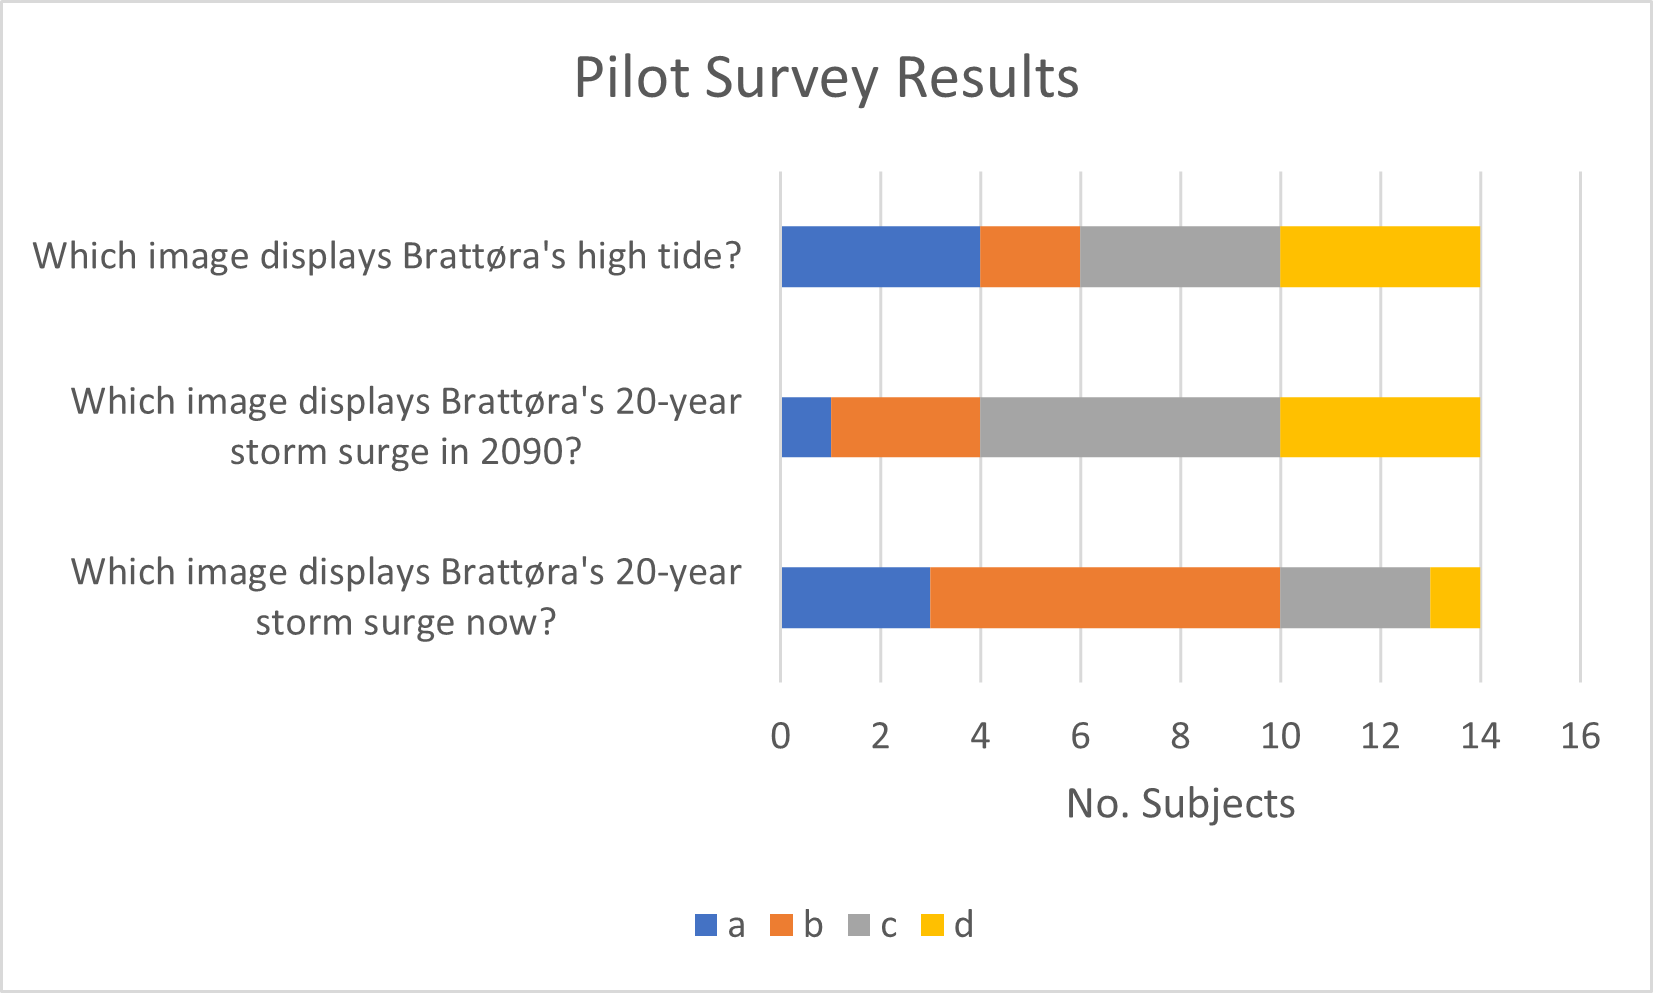
\includegraphics{fig_results/pilot_survey_results.png}
    \caption{Pilot Survey Results}{Staked Bar Chart of Pilot Survey Results - 14 subjects asked three questions about SLEs as displayed in the Methodology section. Answers \textbf{a,b,c,d} correspond to one of the four options for maps of different SLEs in Brattøra as seen in figures \ref{fig:brattora_2022_hightide}, \ref{fig:brattora_2022_stormsurge},and  \ref{fig:brattora_2090_stormsurge}. Answers are colour coded: \textbf{a} is blue, \textbf{b} is orange, \textbf{c} is grey and \textbf{d} is yellow. Response to the first question "Which image displays Brattøra's high tide?"show no observable preference for any of the answers, the answer corresponding with \cite{kartverket_se_2021} was \textbf{c}. The second question "Which image displays Brattøra's 20-year storm surge in 2090" displayed a preference for answer \textbf{c}, the answer corresponding with \cite{kartverket_se_2021} was \textbf{b}. The third question "Which image displays Brattøra's 20-year storm surge now?" has a preference for answer \textbf{b}, the answer corresponding with \cite{kartverket_se_2021} was \textbf{b}.}
    \label{fig:pilot_survey_results}
\end{figure}

Due to this groups assumed high knowledge the lack of correspondence between answers and models as shown in figure \ref{fig:pilot_survey_results} was enough that conducting a focus group was deemed necessary (section \ref{method-pilot}).

Response to the first question "Which image displays Brattøra's high tide?"show no observable preference for any of the answers, the answer corresponding with \cite{kartverket_se_2021} was \textbf{c}. The second question "Which image displays Brattøra's 20-year storm surge in 2090" displayed a preference for answer \textbf{c}, the answer corresponding with \cite{kartverket_se_2021} was \textbf{b} and only 4/14 subjects selected that answer. The third question "Which image displays Brattøra's 20-year storm surge now?" has a preference for answer \textbf{b}, the answer corresponding with \cite{kartverket_se_2021} was \textbf{b} and half of the subjects chose this answer.

\paragraph{}


\subsection{Focus Group Feedback}
Half of the participants from the pilot survey took part in the focus group. The main result from the focus group  was that the maps looked too similar, especially when using smart phones for survey completion. It was difficult to tell the maps apart due to the difficulty to identify the relatively small changes in the waterline. This was particularly the case for the question about the high tide (figure \ref{fig:sle_brattora_num}). Furthermore, several participants highlighted that they did not think of SLEs in terms of the square metres of land which is flooded, but solely in terms of changing height. This one dimensional view (height in metres) was highlighted by the group as a limiting factor in the understanding of potential impacts. 
\paragraph{}

When the focus group were asked which type of visualisation method would be most effective and assist them in answering the questions set in the pilot survey - maps, edited photographs or numerical values (see figure \ref{fig:slide} in methodology section \ref{method-pilot}) - the majority favoured the edited photographs, but several participants favoured the numerical visualisations. Of those that chose numeric value visualisation, there was a recognition that was likely due to their professional background, which included utilising numeric representation of SLEs. Those with a longer knowledge of Trondheim (greater than 2 years) favoured the edited photographs. This was also highlighted as the option with the highest emotional impact and the visualisation which caught the whole focus groups attention.
\paragraph{}






\section{Results from the Survey to Determine Trondheim's Social Systems Resilience}

This section focuses on the results obtained from the survey conducted to determine social systems resilience to SLEs in Trondheim.  It also includes the results from Kruskal Wallis Rank Sum Tests and Shapiro Tests on the collected data. The outputs from the survey questions are graphically visualized and presented. These results will be discussed later to determine Trondheim's social systems resilience to SLEs (section \ref{discussion-framework}). The tables and graphs in the following section make reference to the main research survey questions. The full surveys, both Norwegian and English, are available in appendix C. Reference in the text is only made to the English questions. 



\subsection{Place and Language}
Table \ref{tab:place_language} shows the place and language breakdown of the 153 subjects who completed the main survey. 
\begin{table}[H]
    \centering
    \begin{tabular}{|l|l|l|l|}
    \hline
    \textbf{Place}  & \textbf{ English} & \textbf{Norwegian} & \textbf{Total Subjects}  \\ \hline
      Skansen & 11 & 18  & 29    \\ \hline
      Nidelva & 28 & 29 & 57      \\ \hline
      Grillstad & 13 & 24 & 37       \\ \hline
      Brattøra & 14 & 16 & 30     \\ \hline
      Total & 66 & 87 & 153   \\ \hline
     \end{tabular}
    \caption{Place and Language of of Survey Responses}{ Which language or place did the subjects chose to answer on is displayed in this table. The most popular sub-survey was Nidelva with 57 responses, representing 37 \% of responses. Next popular was Grillstad with 37 responses and then Brattøra with 30 and Skansen with 29 respectively. The reasonable spread of response allows for effective comparison. More subjects responded in Norwegian (87) than English (66), but it was comparably split for each location whether the survey was completed in Norwegian or English. }
    \label{tab:place_language}
\end{table}
\paragraph{}

The most popular place for responses was Nidelva, followed by Grillstad, Brattøra and finally Skansen. Almost evenly split for each location was whether the survey was completed in Norwegian or English. Overall responses in English totalled 66, while the Norwegian surveys had 87 responses.  

\subsection{Interest Level in SLEs}
The following two figures (figure \ref{fig:interest_level_SLE} and figure \ref{fig:aware_vs_interest}) show the results from the survey questions on self-ranking interest level. 80 \% of subjects responded with a medium or higher level of interest. 


\begin{figure}[H]
    \centering
    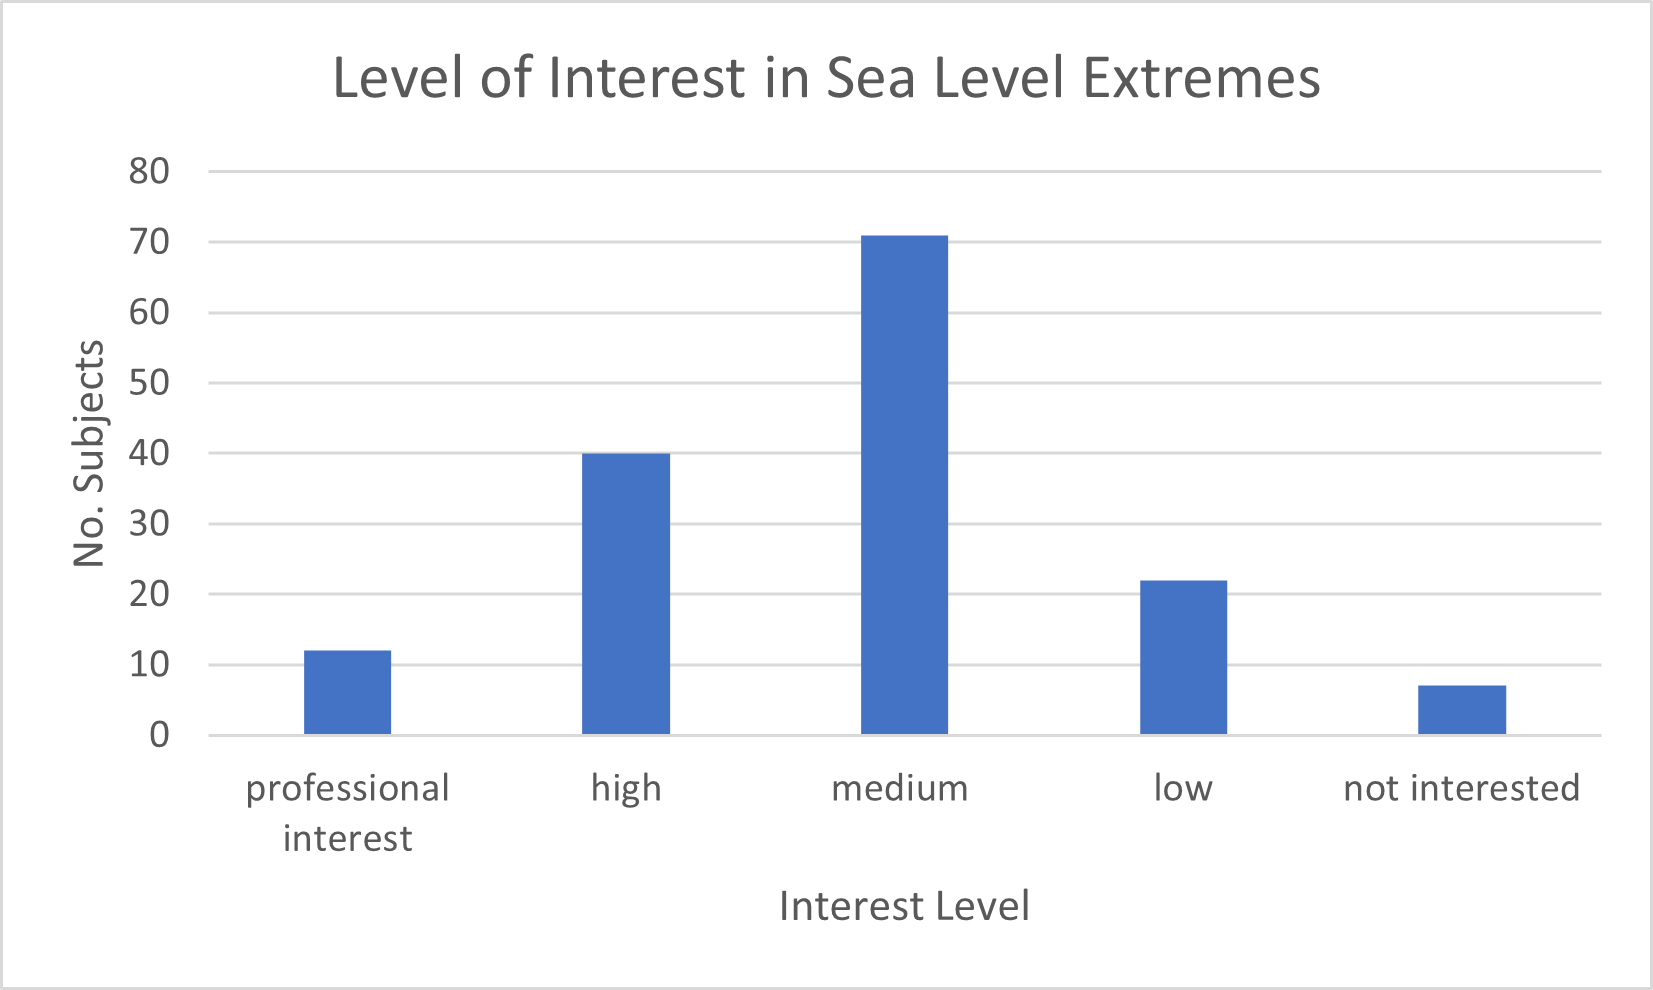
\includegraphics{fig_results/interest-level.png}
    \caption{Interest Level in SLEs are well spread}{22 subjects have low interest in SLEs, 7 are not interested.  Almost half of the subjects (71/153) answered that they have a medium interest in SLEs. More subjects answered that they had a high level of interest (40) than have a low level of interest in SLEs. 12 subjects answered that they have professional interest in SLEs. }
    \label{fig:interest_level_SLE}
\end{figure}
\paragraph{}

The majority of respondents answered that their interest in SLEs is medium. Interestingly, 7 subjects responded that they have no interest, while 12 subjects responded that they have a professional interest in SLEs. 
\paragraph{}
Figure \ref{fig:aware_vs_interest} displays awareness against self-ranking interest level.

\begin{figure}[H]
    \centering
    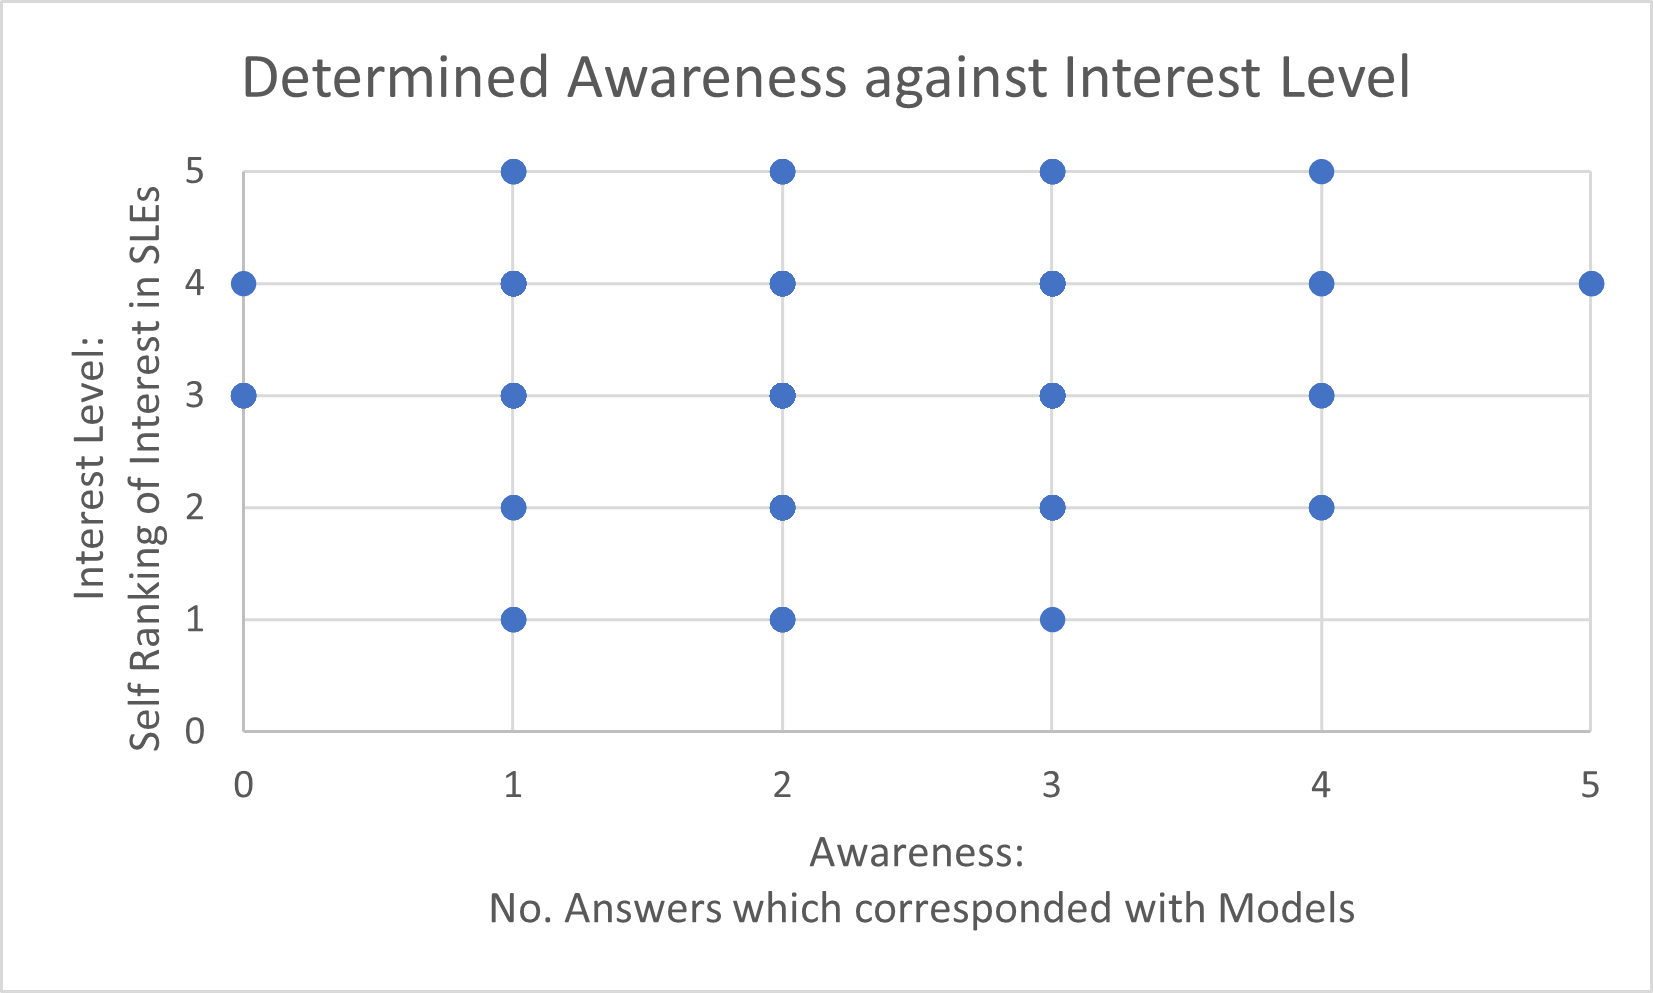
\includegraphics{fig_results/aware_vs_interest.png}
    \caption{Determined Awareness Against Interest Level}{ Professional interest is level 5 on the y-axis, High  is level 4, medium is level 3, 2 is low interest and 1 is not interested. Subjects who responded high levels of interest are determined as representing all levels of awareness.  }
    \label{fig:aware_vs_interest}
\end{figure}
\paragraph{}

There is no linearity or other pattern observed in figure \ref{fig:aware_vs_interest}. Medium level self ranking of interest has almost as broad a variation in awareness as high level, but does not include any subjects who were determined to have the highest level of awareness.  It is worth noting  that figure \ref{fig:aware_vs_interest} does not display how often subjects interest level matched their awareness. A single subject is enough for a blue dot to be displayed as there is no weighting with this figure, though this can be inferred from figure \ref{fig:interest_level_SLE}. 


\subsection{Memory of SLEs and Length of Place-based Knowledge}
The spread of the memory of sea level extreme events in Trondheim by the subjects is shown in figure \ref{fig:memory_sle}.

\begin{figure}[H]
    \centering
    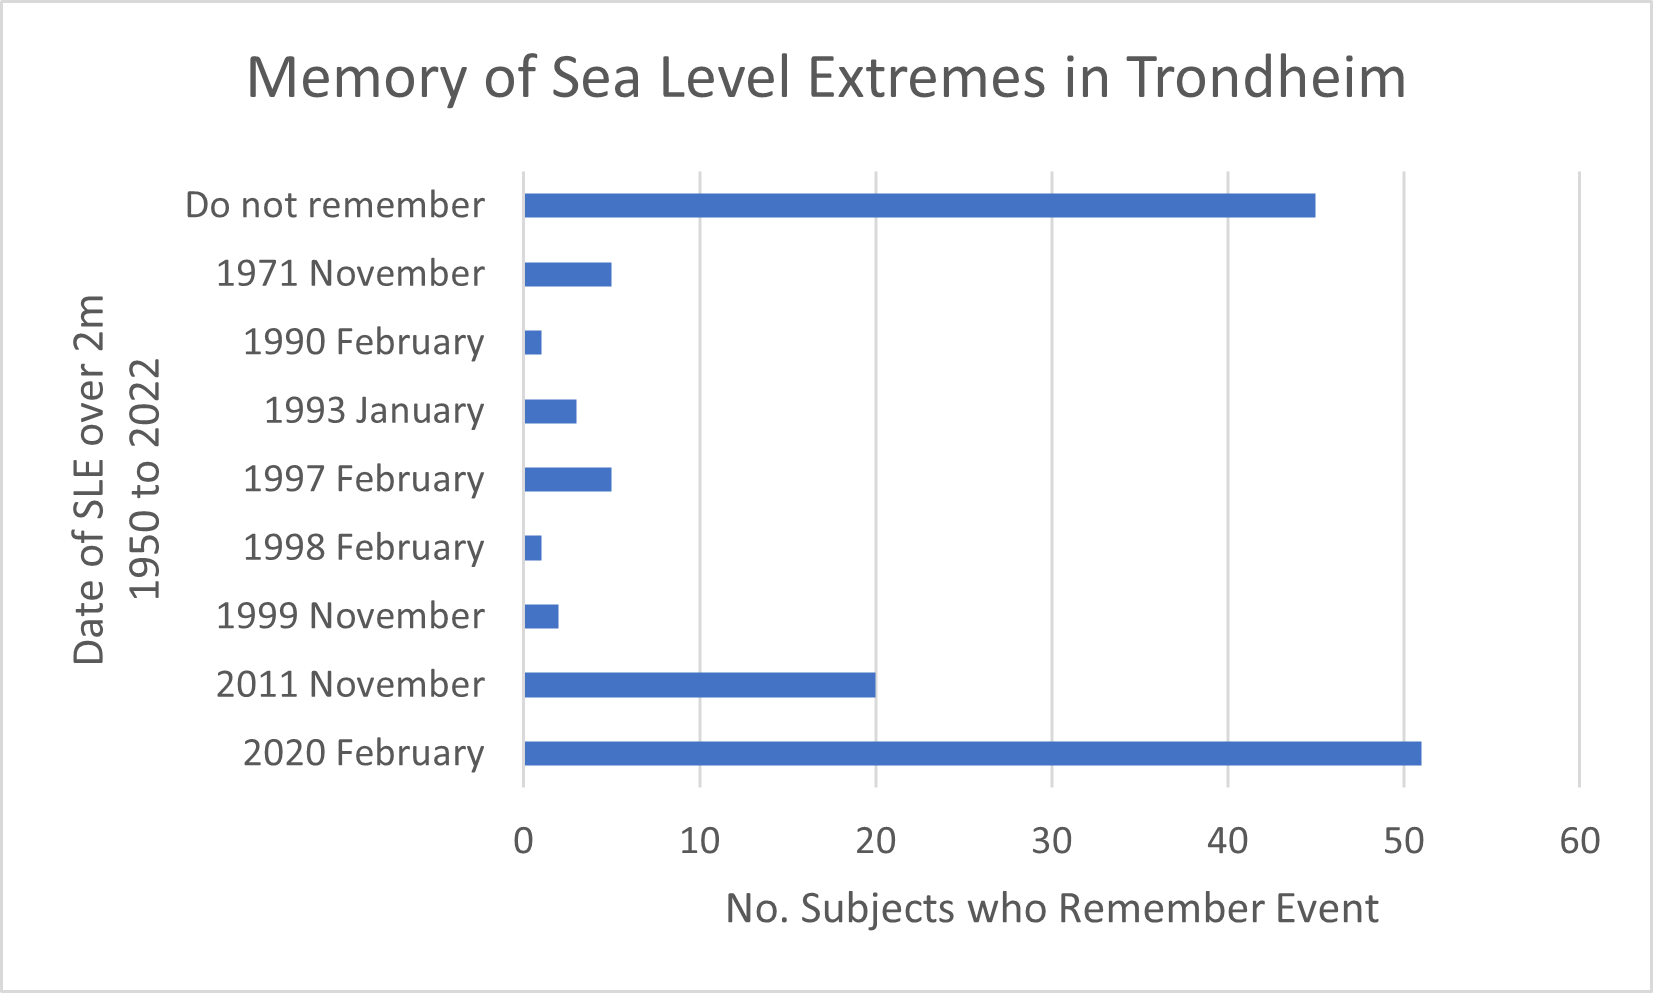
\includegraphics{fig_results/memory-sle.png}
    \caption{Memory of SLEs}{ The subjects were asked which SLE events (water level higher than 2m) they remembered occurring between 1950 and summer 2022. For the full list of potential events please consults appendix C. 45 out of 153 subjects (30\%) do not remember any sea level extreme event in Trondheim. Only one subject remembered every sea level extreme event dating back to 1950 in Trondheim. 51 subjects remembered the sea level extreme event in February 2020. }
    \label{fig:memory_sle}
\end{figure}
\paragraph{}

Memory has a very skewed factor, 30\% of subjects have no memory of SLEs in Trondheim. Once the response of "Do not remember" is excluded, there is almost an exponential increase in the number of subjects who remember the SLE events, with the most common result being the most recent SLE event where the water level was higher than 2m.  
\paragraph{}
Figure \ref{fig:long_know} shows the responses to the place-based length of knowledge question.

\begin{figure}[H]
    \centering
    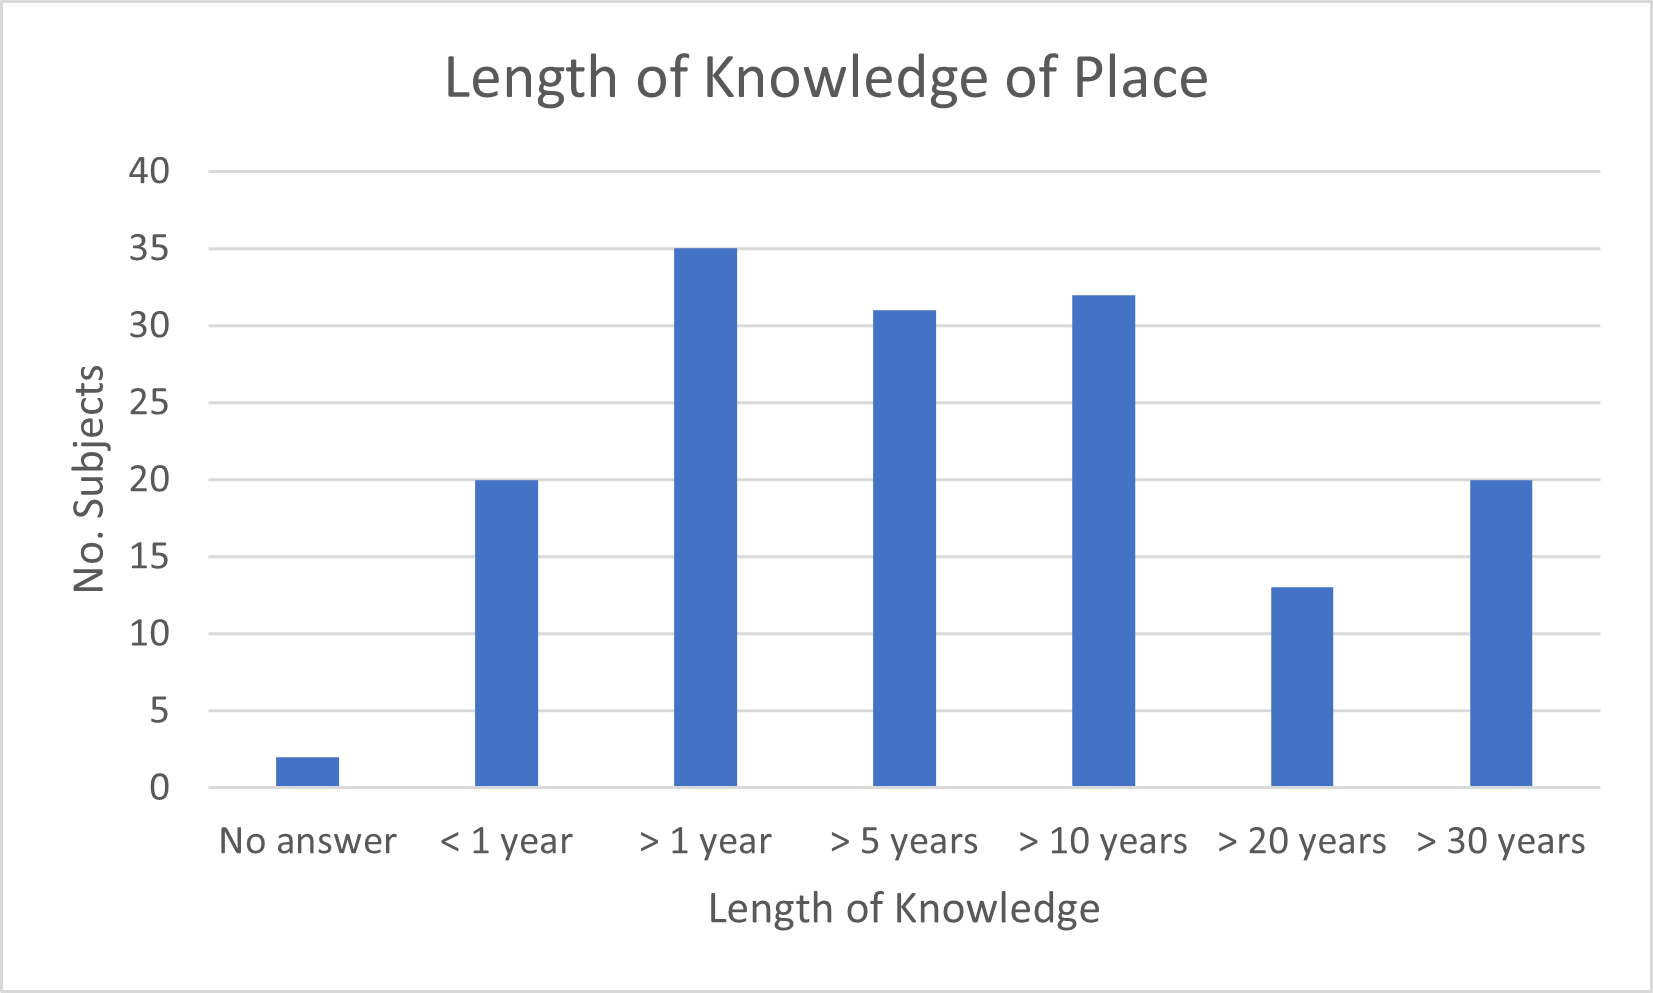
\includegraphics{fig_results/long_know.png}
    \caption{Length of Knowledge of Subjects.}{ 96 subjects had a length of knowledge about the place greater than 5 years 35 subjects had length of knowledge less than 5 years, but more than 1. Only 20 respondents had a length of knowledge under 1 year about the place they chose to answer on.}
    \label{fig:long_know}
\end{figure}

20 subjects responded that they had a length of knowledge of Trondheim under one year. 96 subjects responded that they had a length of knowledge greater than five years, which includes the sea level extreme event occurring in February 2020, which only 51 subjects remembered (figure \ref{fig:memory_sle}). The difference between a SLE event and a disaster and how this impacts memory and resilience is expanded upon in the discussion (section \ref{discuss-memory}).



\subsection{Information Access about Climate and Place}

There is significant skew in how subjects access information about climate and place as can be seen in table \ref{table:sum_stats_info_climate_access} and table \ref{table:sum_stats_info__place_access} below. That individuals with a broader range of information sources have higher levels of awareness is one of the hypotheses outlined in the introduction (section \ref{hypotheses-intro}). 

\begin{center}
\begin{table}[H]
    \centering
    \begin{tabular}{|l|l|l|l|l|l|l|}
    \hline
        \textbf{Factor} & \textbf{mean} & \textbf{Std Dev}. & \textbf{ min} & \textbf{max} & \textbf{ range} & \textbf{skew}  \\ \hline
        
      Sum of Information Access & 3.50 & 1.72 & 0 & 8 & 8 & 0.24 \\ \hline
        Personal Observation  & 0.45 & 0.50 & 0 & 1 & 1 & 0.20 \\ \hline
        Family & 0.18 & 0.38 & 0 & 1 & 1 & 1.68  \\ \hline
        Friends & 0.23 & 0.42 & 0 & 1 & 1 & 1.28  \\ \hline
        Newspapers & 0.72 & 0.45 & 0 & 1 & 1 & -0.96 \\ \hline
        TV & 0.46 & 0.50 & 0 & 1 & 1 & 0.14 \\ \hline
        Social Media & 0.63 & 0.48 & 0 & 1 & 1 & -0.55 \\ \hline
        Membership of Organisations & 0.14 & 0.35 & 0 & 1 & 1 & 2.09 \\ \hline
       Peer Reviewed Publications & 0.39 & 0.49 & 0 & 1 & 1 & 0.44 \\ \hline
        Formal Education & 0.29 & 0.46 & 0 & 1 & 1 & 0.89 \\ \hline
        
         \end{tabular}
    \caption{Information Source about Climate Summary Statistics }{Factors: Sum of Information Access (how many sources a subject selected, 1-8), Personal Observation, Family, Friends, Newspapers, TV, Social Media, Membership of Organisations, Peer Reviewed Publications, Formal Education.
    \paragraph{}
    Mean - average, i.e. the total of the values, divided by the sum of these values. 
    Std Dev. - standard deviation, i.e. on average, how far each value lies from the mean.
    Min - minimum, i.e. the smallest value in this case representing an non-selected response hence 0.
    Max - maximum i.e the largest value, for the majority of factors this is 1, but for Sum of Information Access this is 8.
    Range - difference between the minimum and maximum i.e. the largest value minus the smallest value
    Skew - measure of the asymmetry of the results, equal distribution has a skew of 0.}
\label{table:sum_stats_info_climate_access}
\end{table}
\end{center}

\begin{center}
\begin{table}[H]
    \centering
    \begin{tabular}{|l|l|l|l|l|l|l|}
    \hline
         \textbf{Factor} & \textbf{mean} & \textbf{Std Dev.} & \textbf{min} & \textbf{max} & \textbf{range} & \textbf{skew}  \\ \hline
        Sum of Information Access & 1.94 & 1.34 & 0 & 8 & 8 & 1.61 \\ \hline
        Personal Observation & 0.73 & 0.45 & 0 & 1 & 1 & -1.00  \\ \hline
        Family & 0.10 & 0.31 & 0 & 1 & 1 & 2.56 \\ \hline
        Friend & 0.19 & 0.39 & 0 & 1 & 1 & 1.57  \\ \hline
        Newspaper & 0.35 & 0.48 & 0 & 1 & 1 & 0.64  \\ \hline
        TV & 0.14 & 0.35 & 0 & 1 & 1 & 2.09 \\ \hline
       Social Media & 0.33 & 0.47 & 0 & 1 & 1 & 0.73  \\ \hline
        Membership of Organisations & 0.04 & 0.19 & 0 & 1 & 1 & 4.70 \\ \hline
        Trondheim Municipality & 0.07 & 0.26 & 0 & 1 & 1 & 3.28\\ \hline
                
         \end{tabular}
    \caption{Information Source about Place Summary Statistics}{Factors: Sum of Information Access (how many sources a subject selected, 1-8), Personal Observation, Family, Friends, Newspapers, TV, Social Media, Membership of Organisations, Trondheim Municipality. 
    \paragraph{}
    Mean - average, i.e. the total of the values, divided by the sum of these values. 
    Std Dev. - standard deviation, i.e. on average, how far each value lies from the mean.
    Min - minimum, i.e. the smallest value in this case representing an non-selected response hence 0.
    Max - maximum i.e the largest value, for the majority of factors this is 1, but for Sum of Information Access this is 8.
    Range - difference between the minimum and maximum i.e. the largest value minus the smallest value
    Skew - measure of the asymmetry of the results, equal distribution has a skew of 0.}
\label{table:sum_stats_info__place_access}
\end{table}
\end{center}
Social media is the most common source of information used to access information about climate change, but a less popular source for information about place. Membership of organisations is the least popular source of information for both climate and place information. Personal observation is the most popular source for information about place and the fourth most popular source for information about climate. On average, subjects selected more sources for information about climate than information about place (Mean sum of information access information about climate is 3.50, while the mean sum of information access about place is 1.95.) 
\paragraph{}
These highly skewed responses with a large variation in mean and standard deviation impacted the type of hypothesis testing which could be carried out as discussed in section \ref{method-data-analysis}. The lack of linearity, and asymmetrical distribution meant a non parametric hypothesis testing method was chosen, specifically the Kruskal Wallis Rank Sum Test.

\subsection{Community Membership}
Stakeholders targeted were those with direct experience of the four research sites either by living, commuting or working in coastal Trondheim. As stated in the Methodology (section \ref{data-collection}), subjects were asked to identify themselves as members of communities that were highlighted by a stakeholder analysis. They were also given the choice to write in other community membership if they selected other. Figure \ref{fig:community_membership} displays the community memberships selected by the subjects. 

\begin{figure}[H]
    \centering
    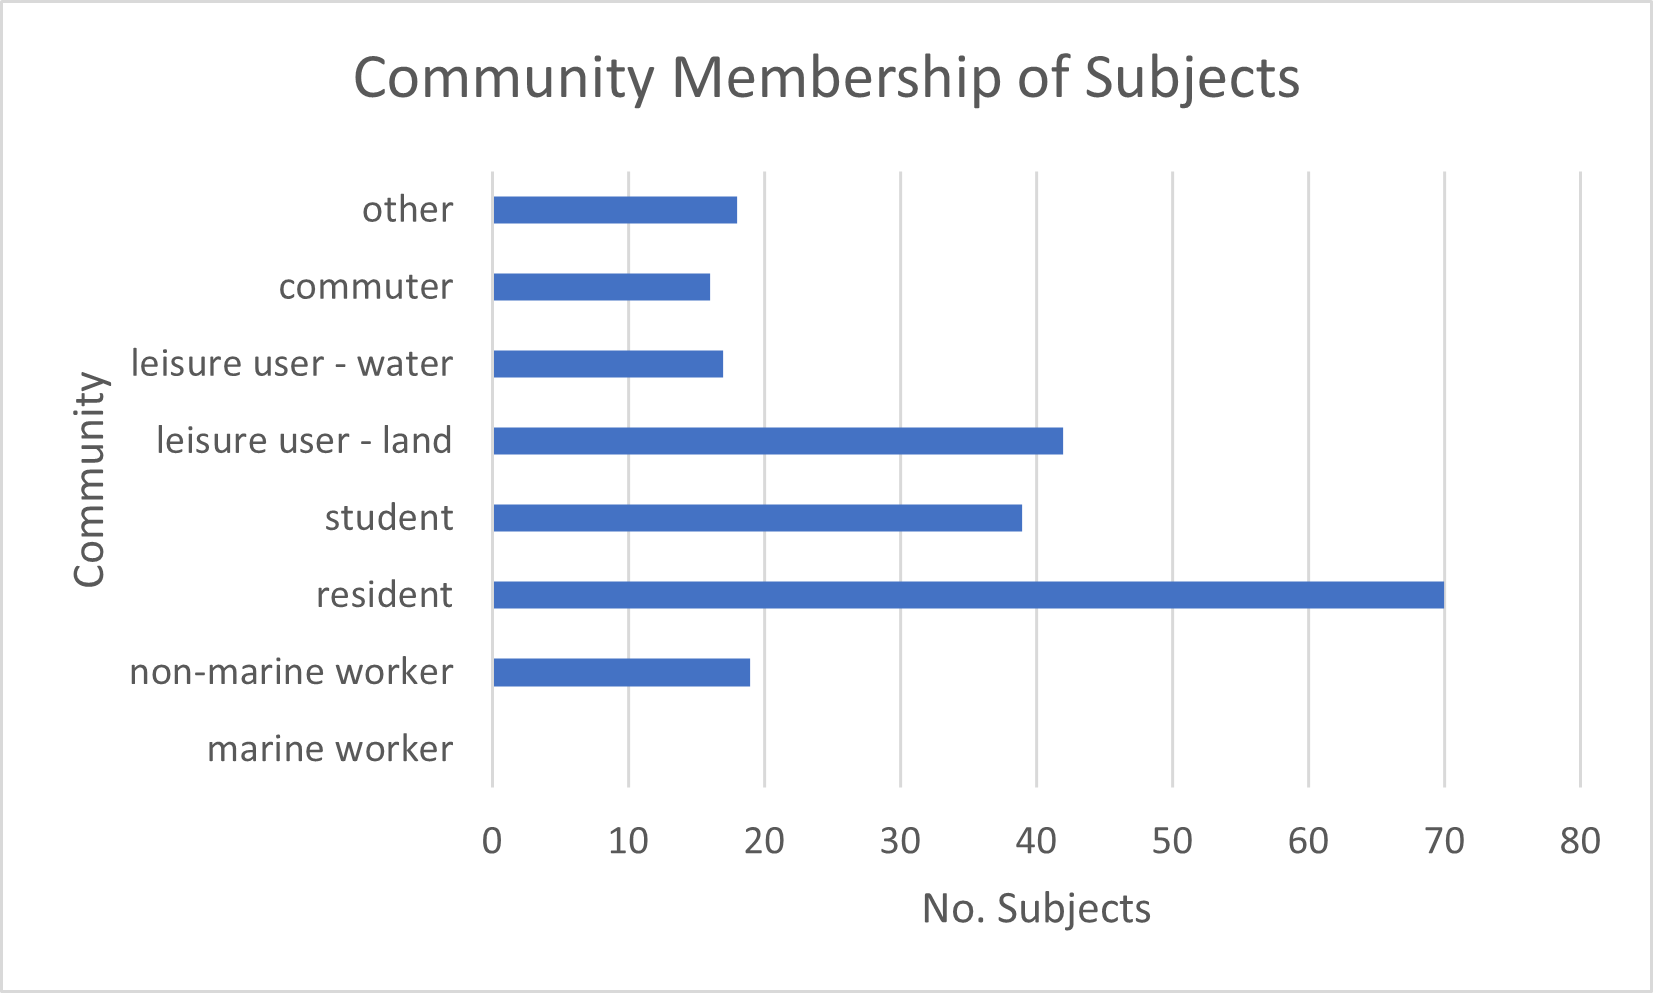
\includegraphics{fig_results/com-mem-horizontal.png}
    \caption{Membership of Communities}{ There were 221 selections done by the 153 subjects. However many subjects only selected one community. The most selected community was resident, 70 out of 153 subjects - under half of the subjects. Next most popular is leisure user -land, followed by student. No subjects responded with marine worker. }
    \label{fig:community_membership}
\end{figure}
\paragraph{}

There are 70 subjects who answered that they are residents. This is the most common choice. Very few subjects who answered they were students also selected a second community membership. Subjects who answered as other were either visitors, tourists or sailors. No subjects responded as marine workers. The impact of subjects only selecting a single response in this format of question is discussed in the discussion of framework (section \ref{discuss-additional-considerations}. 


\subsection{Access to Survey}
Figure \ref{fig:survey_access} shows how subjects accessed the survey.  

\begin{figure}[H]
    \centering
    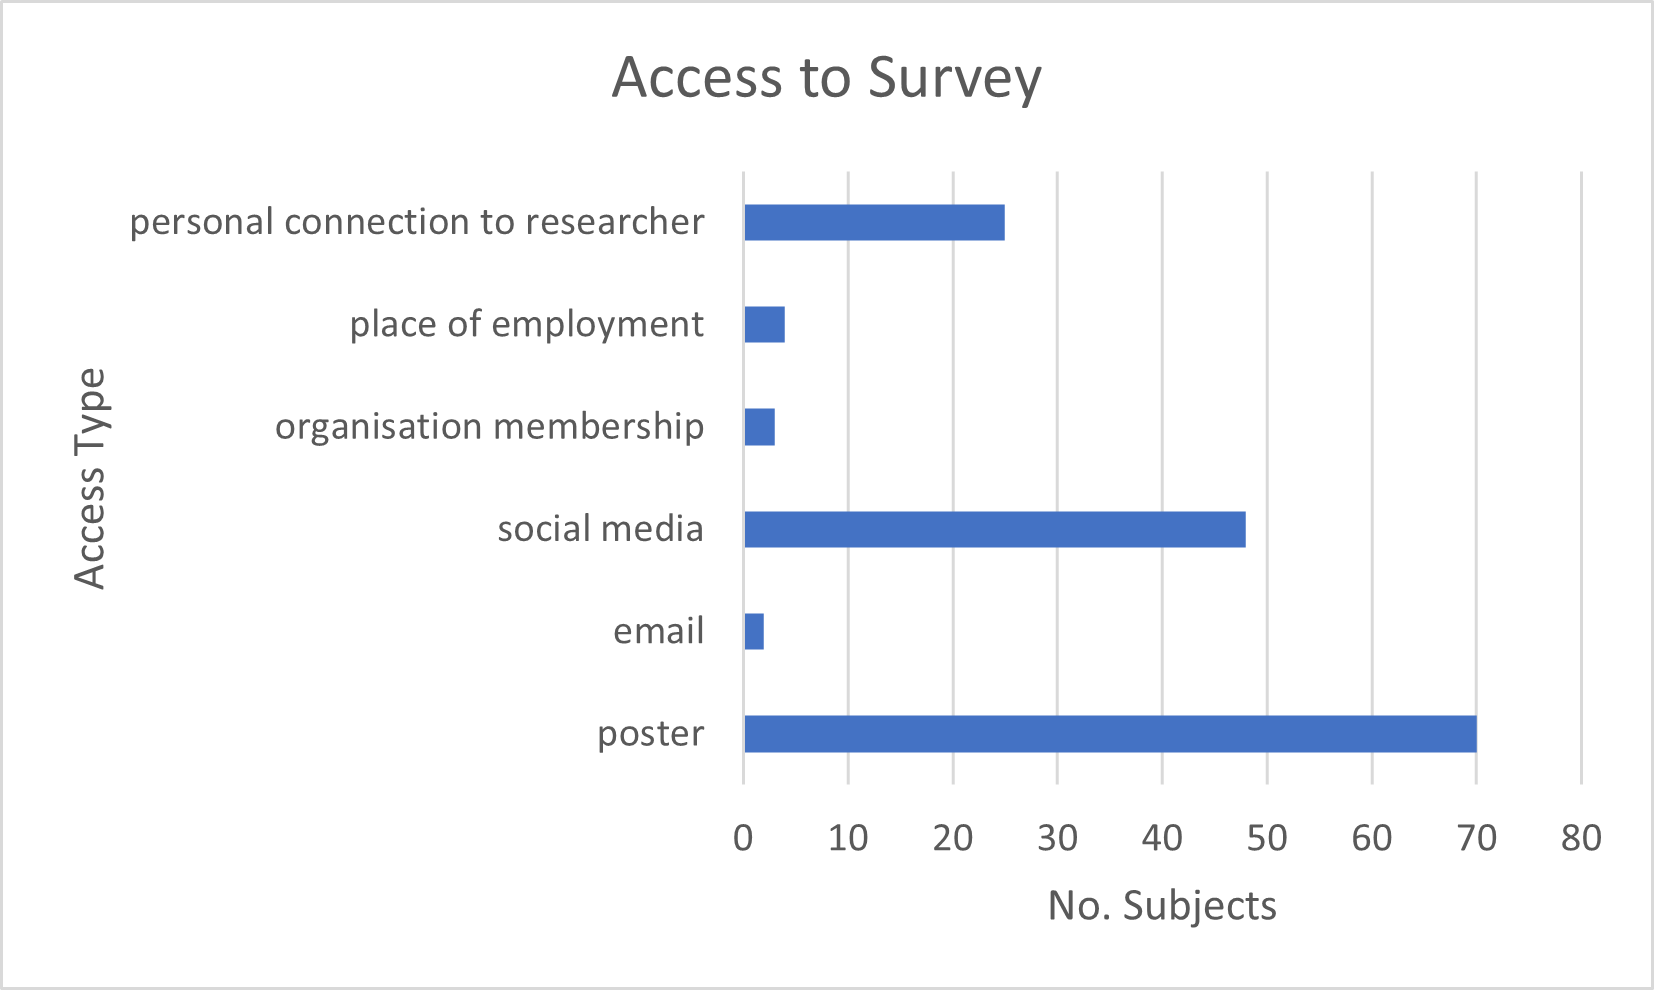
\includegraphics{fig_results/access_survey.png}
    \caption{Access to Survey}{ Six access types were included: personal connection to researcher; place of employment; organisation membership; social media; email; poster. The most popular access method was poster with 70 subjects selecting this response followed by social media}
    \label{fig:survey_access}
\end{figure}
\paragraph{}


The most common access method of the survey was poster, with 70 subjects selecting this choice. This is followed by social media which has 47 subjects choosing this. 25 subjects accessed the survey due to personal connection to researcher. Accesses via email, place of employment and organisation membership all have under 10 subjects. Subjects could chose more than one access type. For example, a subject could have accessed via personal connection to researcher and social media, due to the researcher sharing this survey on their personal social media.  
\paragraph{}



\subsection{Perceived Risks}
How stakeholders perceive risks impacts their social resilience (section \ref{theory-resilience}). Several questions were asked to gauge subjects risk perception especially of personal impacts of SLEs and associated flooding. The first question was "How would flooding associated with sea level extremes in this area affect you?", the results of which are shown in figure \ref{fig:flood_impact_pred}. This survey question was followed with an opportunity to give more details, which is discussed in section \ref{discuss-percieved.risk}.

\begin{figure}[H]
    \centering
    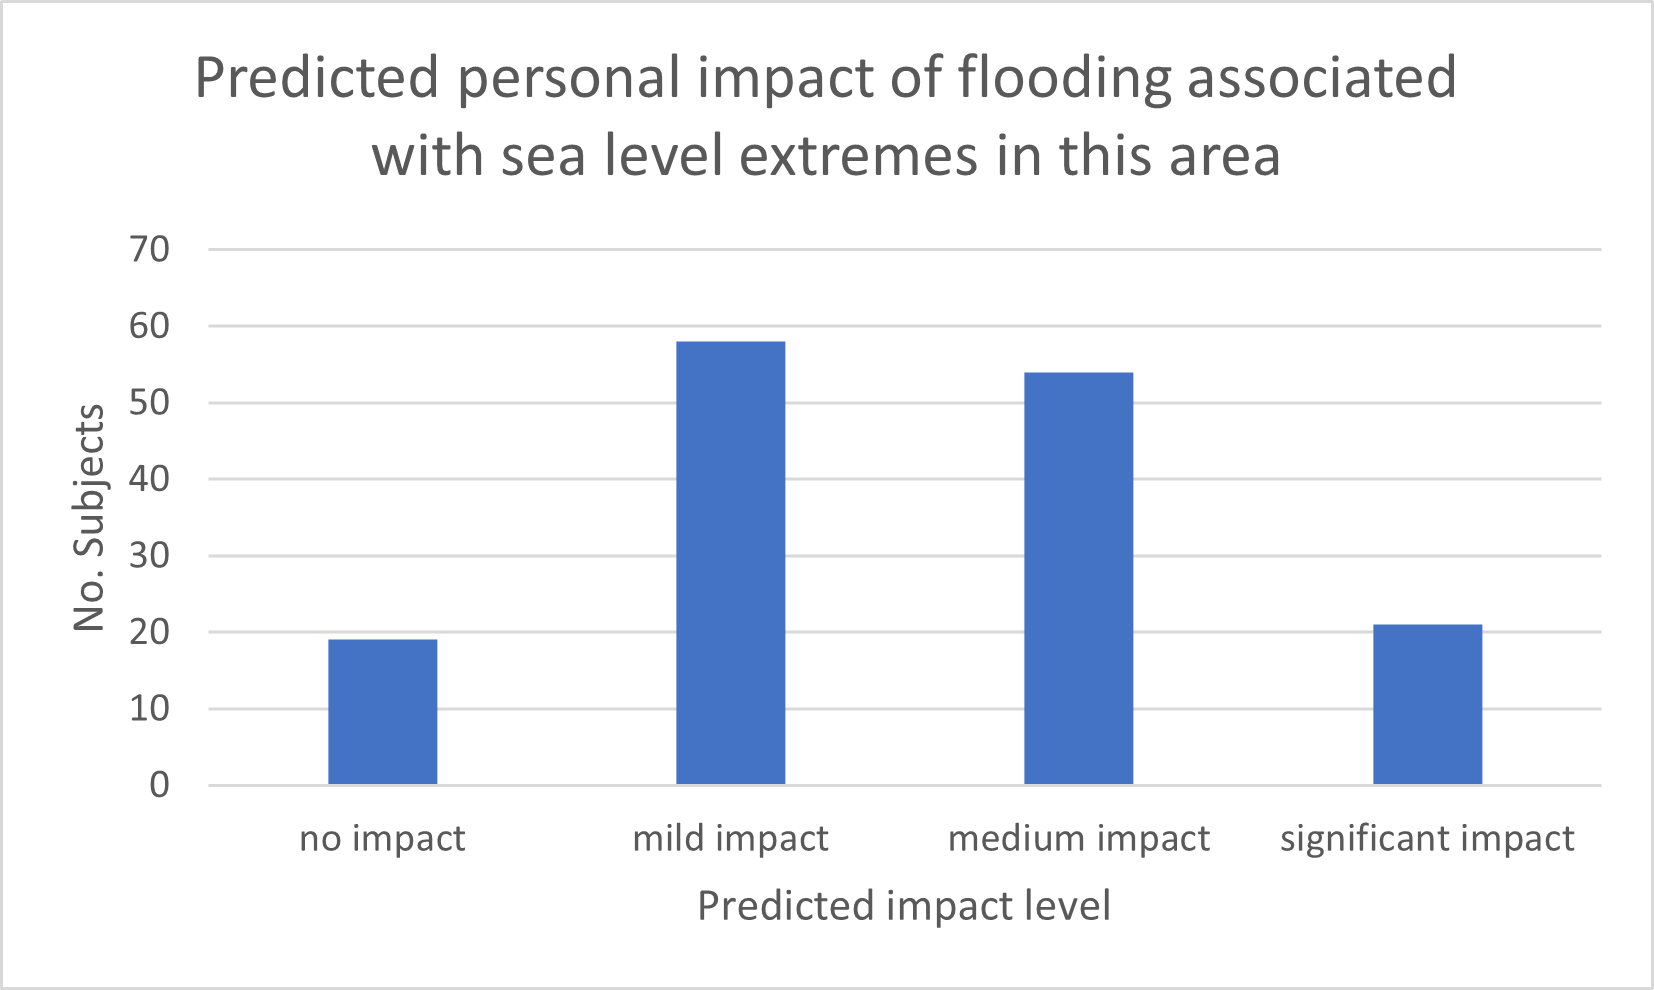
\includegraphics{fig_results/impact-flood-answers.png}
    \caption{Perceived Potential Flood Impact}{
    19 subjects response was that they predicted no impact of flooding associated with SLEs in the research site. While 58 subjects responded mild impact and 54 subjects responded with medium impact. No impact was a less popular response that significant impact, which had 21 responses. A total of 152 responses were collected for this question. }
    \label{fig:flood_impact_pred}
\end{figure}

Figure \ref{fig:flood_impact_pred} is well distributed, with mild impact the most popular response with 38\% of subjects selecting this response. 
\paragraph{}

The second last question in the survey asks "From the following what are the major risks to infrastructure in this area?" (appendix C). Figure \ref{fig:risk_infrastructure} shows the breakdown of subjects' responses about perceived risk to infrastructure. Figure \ref{fig:risk_people}) shows the breakdown of subjects responses about perceived risk to people, the results from the third last question (appendix C).

\begin{figure}[H]
    \centering
    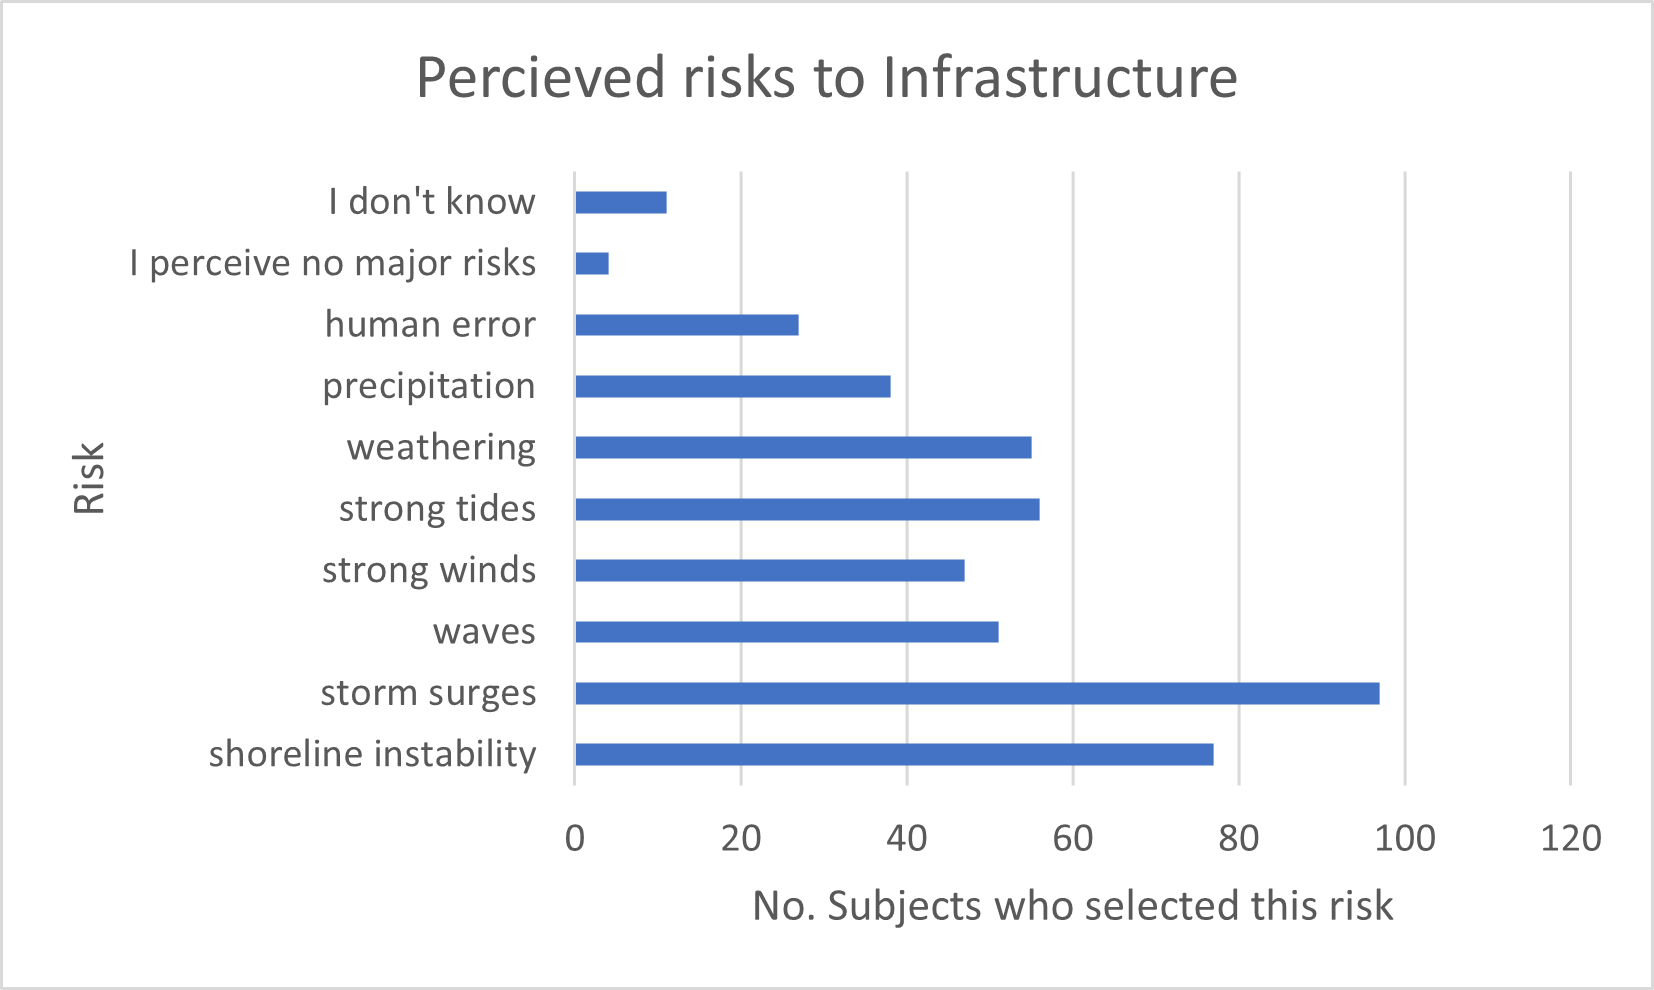
\includegraphics{fig_results/percieved risks to infrastructure.png}
    \caption{Perceived Risks to Infrastructure Risks}{ 97 subjects selected storm surges as a risk to infrastructure. Only 4 subjects responded that they perceived no major risks to infrastructure and 11 subjects responded that they don't know. Human error was only selected by 27 subjects making it the risk the least number of subjects were concerned about. There is greater perception of weather impacts on infrastructure with 47 subjects highlighting strong winds, 51 subjects selecting waves, 56 subjects selecting strong tides and 38 selecting precipitation. After storm surges, which were mentioned multiple times in the survey, there is a perception of shoreline instability as a significant risk with 77 subjects selecting it as a risk to infrastructures.  The total number of responses is 463. }
    \label{fig:risk_infrastructure}
\end{figure}
\paragraph{}


\begin{figure}[H]
    \centering
    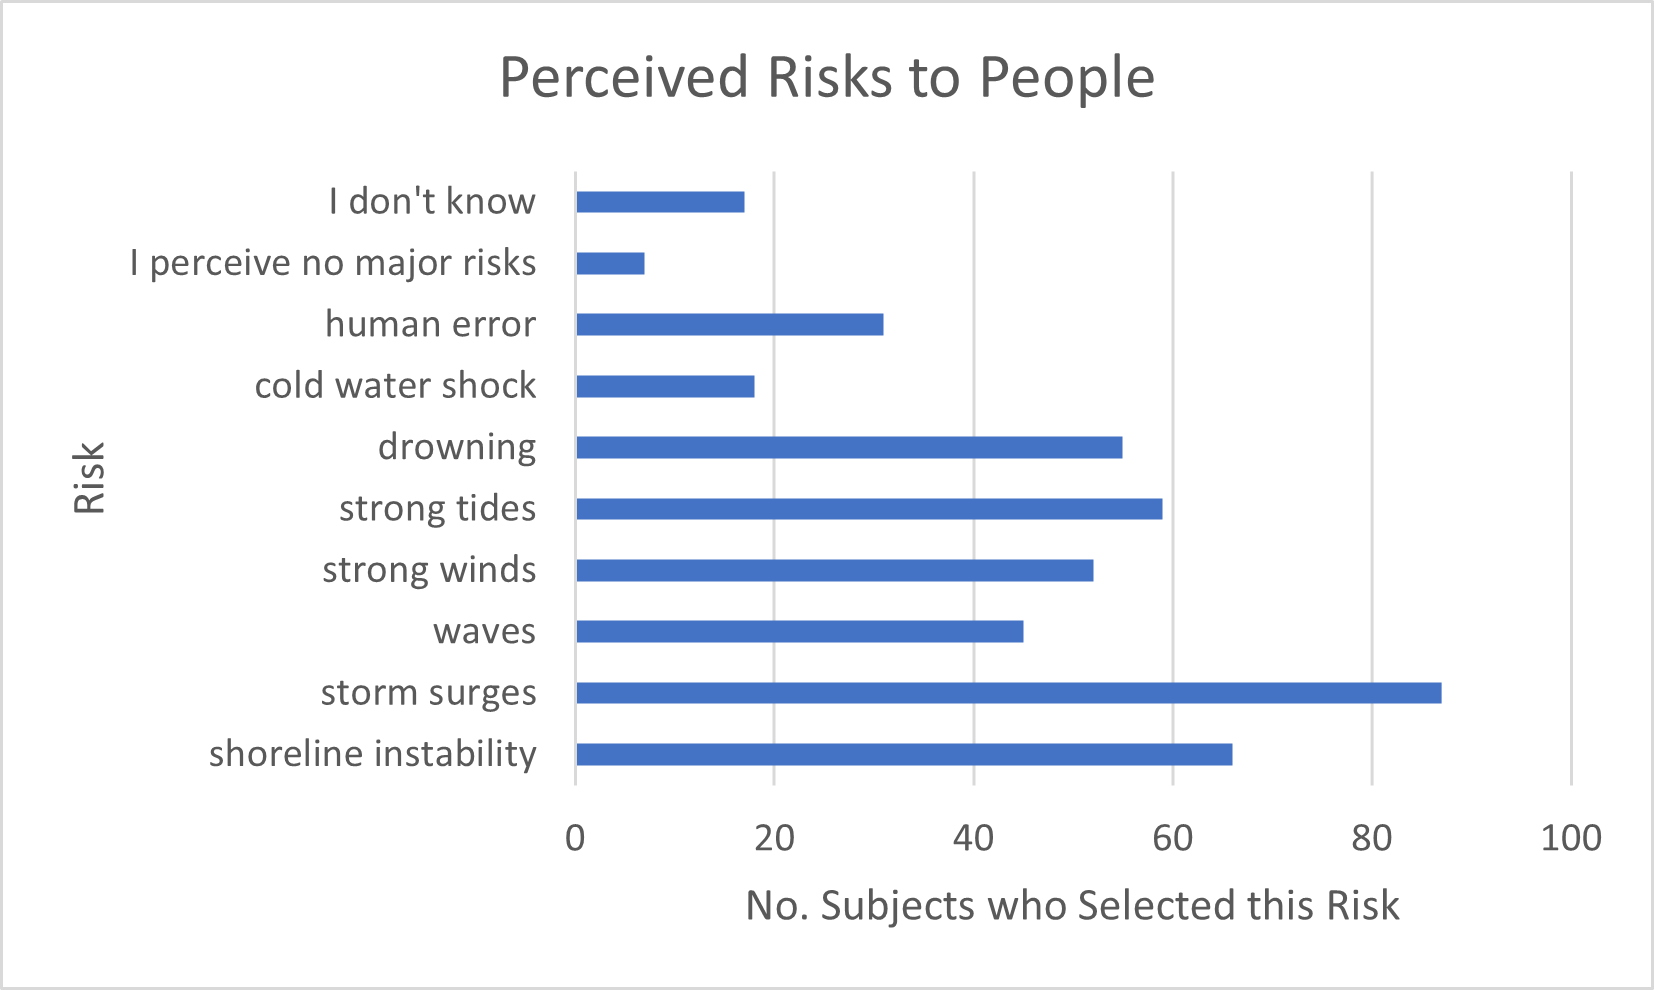
\includegraphics{fig_results/percieved risks to people.png}
    \caption{Perceived Risks to People}{ (87 subjects selected that they perceive storm surges as a risk to people in the research sites. 7 subjects responded that they perceived no major risks to infrastructure and 17 subjects responded that they don't know. Cold water shock was only selected by 18 subjects making it the risk the least number of subjects were concerned about, followed up by human error with 31 subjects. 55 subjects selected drowning as a risk to people in the area of the research sites. While 52 subjects selected strong winds, 45 subjects selected waves and 59 subjects selected strong tides. After storm surges which were mentioned multiple times in the survey there is a perception of shoreline instability as a significant risk with 66 subjects selecting it as a risk to infrastructures.  Total number of responses is 437.
    
    }
    \label{fig:risk_people}
\end{figure}
\paragraph{}
It is interesting that more than 80 subjects have selected storm surges as a risk to infrastructure or people. Shoreline instability is also a very common response across both questions. It is notable that the vast majority of subjects do identify risks to people and infrastructure for these places when offered answers. The response of "I don't know" is more common that the "I perceive no major risks". 


\section{Determination of Subjects' Awareness}
Figure \ref{fig:high_tide_answer} shows that the subjects displayed a high awareness of the tides in Trondheim. In the next five figures (figure \ref{fig:high_tide_answer} to figure \ref{fig:slr_past}) colour coded staked bar charts will be used to display how many subjects agree with \cite{kartverket_se_2021} models. The colour orange indicated the subject selected an answer which corresponds, the colour blue indicates the subject selected an answer which did not correspond with the models. Whether local knowledge corresponds with the models from \cite{kartverket_se_2021}, is important when identifying areas for improving resilience in Trondheim.

\begin{figure}[H]
    \centering
    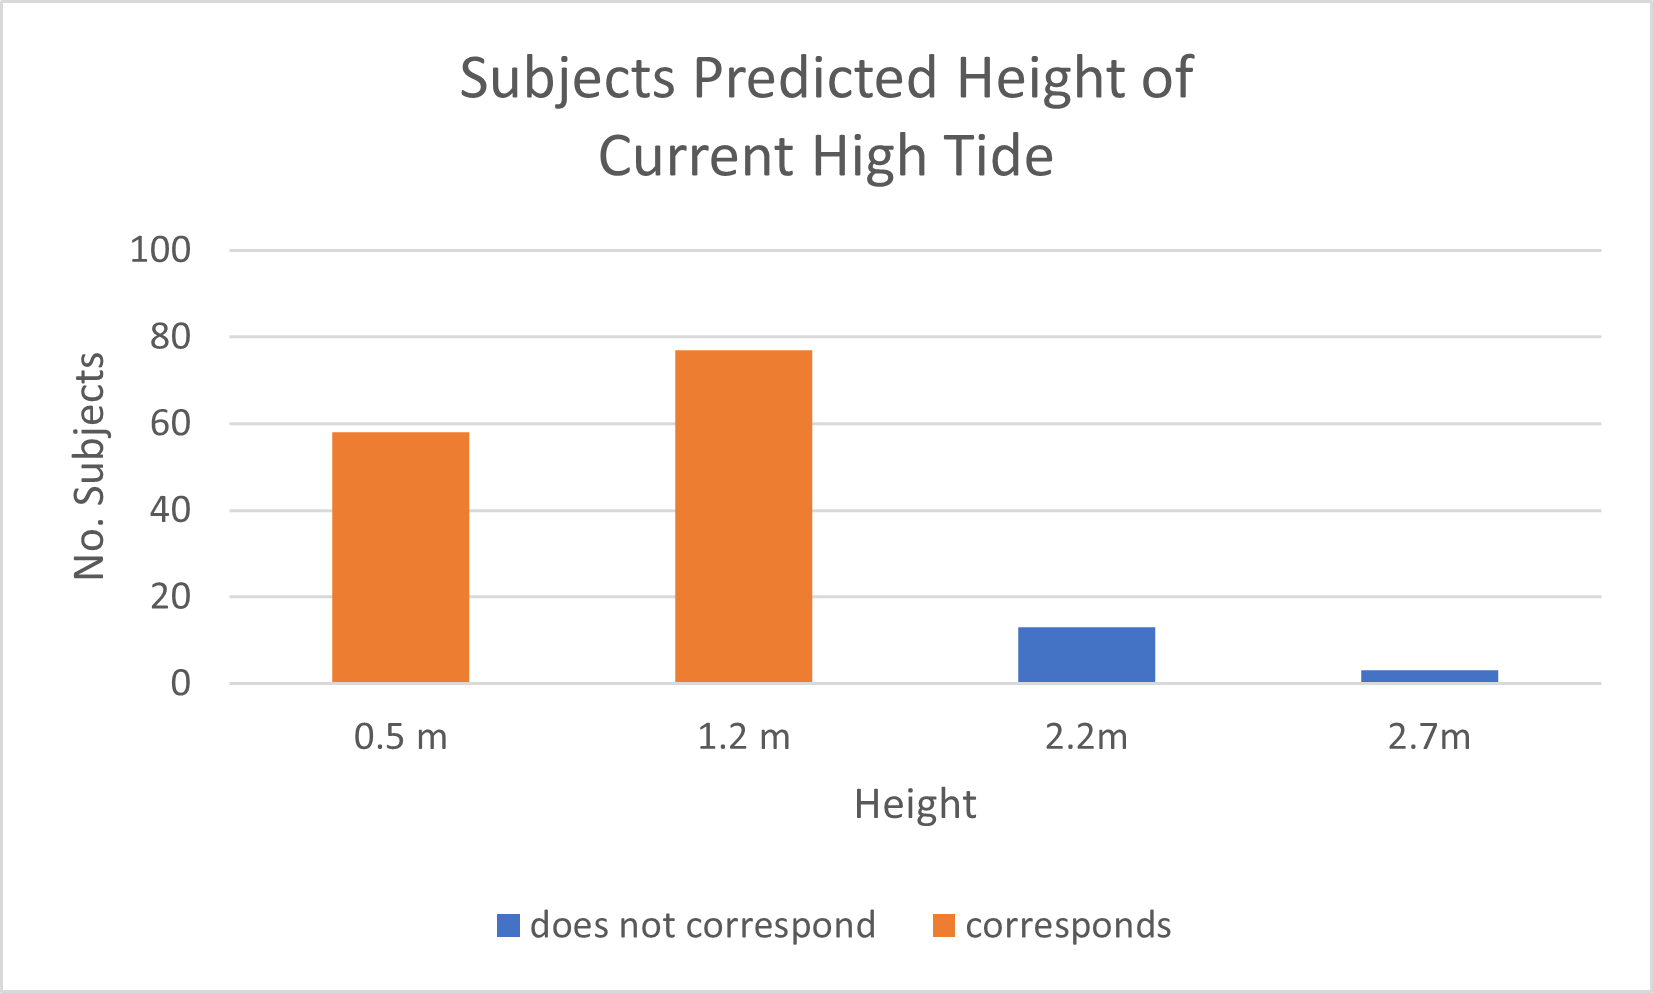
\includegraphics{fig_results/2022-hightide-answers.png}
    \caption{Subjects Predicted Height of Current High Tide}{ Height 0.5m is the neap high tide, Height 1.2m is the spring high tide. The vast majority of subjects selected a value which corresponds with models of tides in Trondheim (\cite{kartverket_se_2021}). 58 subjects chose 0.5m, 77 subjects chose 1.2m meaning that 135 out of 153 subjects (88 \%) chose an answer which could be considered the correct answer for high tide. Only 13 subjects chose 2.2m and 3 subjects chose 2.7m, meaning only 10\% chose an answer which could be considered the incorrect answer for high tide.}
    \label{fig:high_tide_answer}
\end{figure}
\paragraph{}

The height chosen largely corresponds with either the spring or neap high tide - over 80 \% of subjects chose a value which corresponds with the models from (\cite{kartverket_se_2021}). Under 20 subjects responded with a value which does not reflect the models from (\cite{kartverket_se_2021}). The determination of high tide is based on recordings from the tide gauge, hence these values are very reliable (\cite{kartverket_se_2021}).
\paragraph{}
Figure \ref{fig:2022-stormsurge-answers} shows the responses to the question on the predicted height of the current 20 year storm surge. 
\begin{figure}[H]
    \centering
    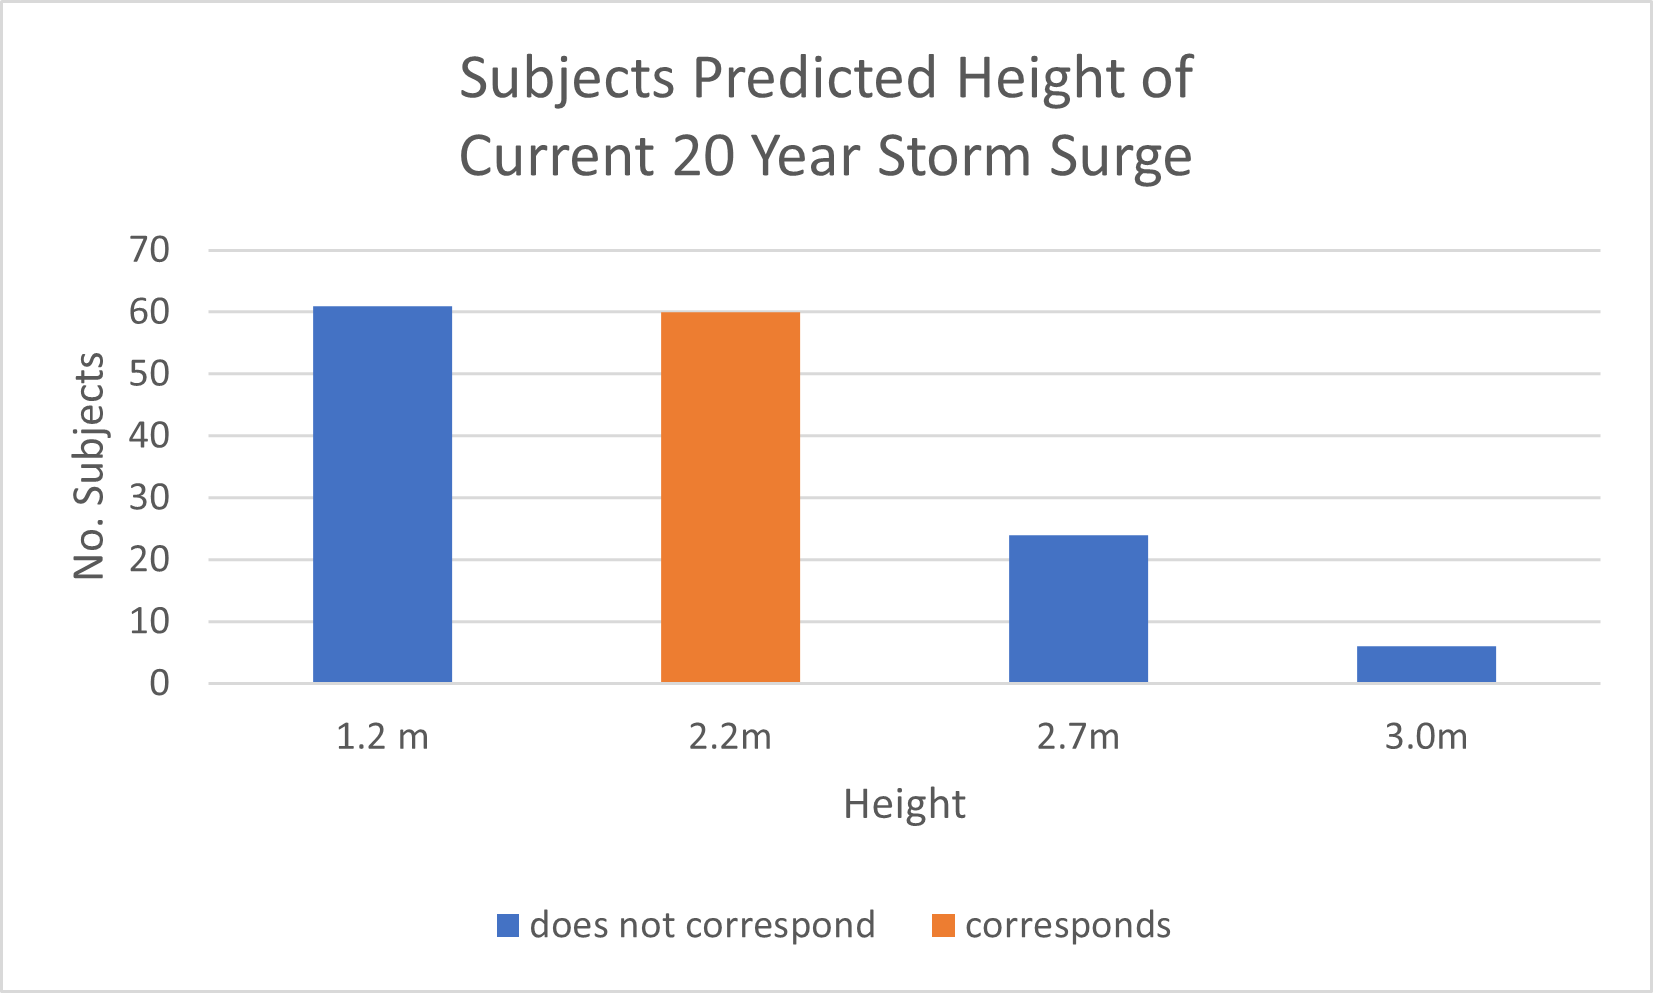
\includegraphics{fig_results/2022-20yrss-answer.png}
    \caption{Subjects Predicted Height of Current 20 Year Storm Surge}{ 61 subjects chose 1.2m this is very comparable to the 60 which chose 2.2m which is the answer which corresponds with (\cite{kartverket_se_2021}). 24 subjects chose 2.7m and only 6 subjects chose 3.0m}
    \label{fig:2022-stormsurge-answers}
\end{figure}
\paragraph{}
The majority of subjects chose 1.2m as the predicted height of the 20 year storm surge, but this does not correspond with models from (\cite{kartverket_se_2021}). In fact, 1.2m is equal to the current high tide. Almost equally often chosen was the answer which does correspond with models from (\cite{kartverket_se_2021}), 2.2m, with 60 subjects choosing this answer. This means that 43 \% of subjects chose the answer which corresponds with (\cite{kartverket_se_2021}). Around 20 \% (30/153) of subjects chose a value higher than the models indicate.
\paragraph{}

Figure \ref{fig:2090-stormsurge-answers} shows the responses to the question on the predicted height of the 2090s' 20 year storm surge.

\begin{figure}[H]
    \centering
    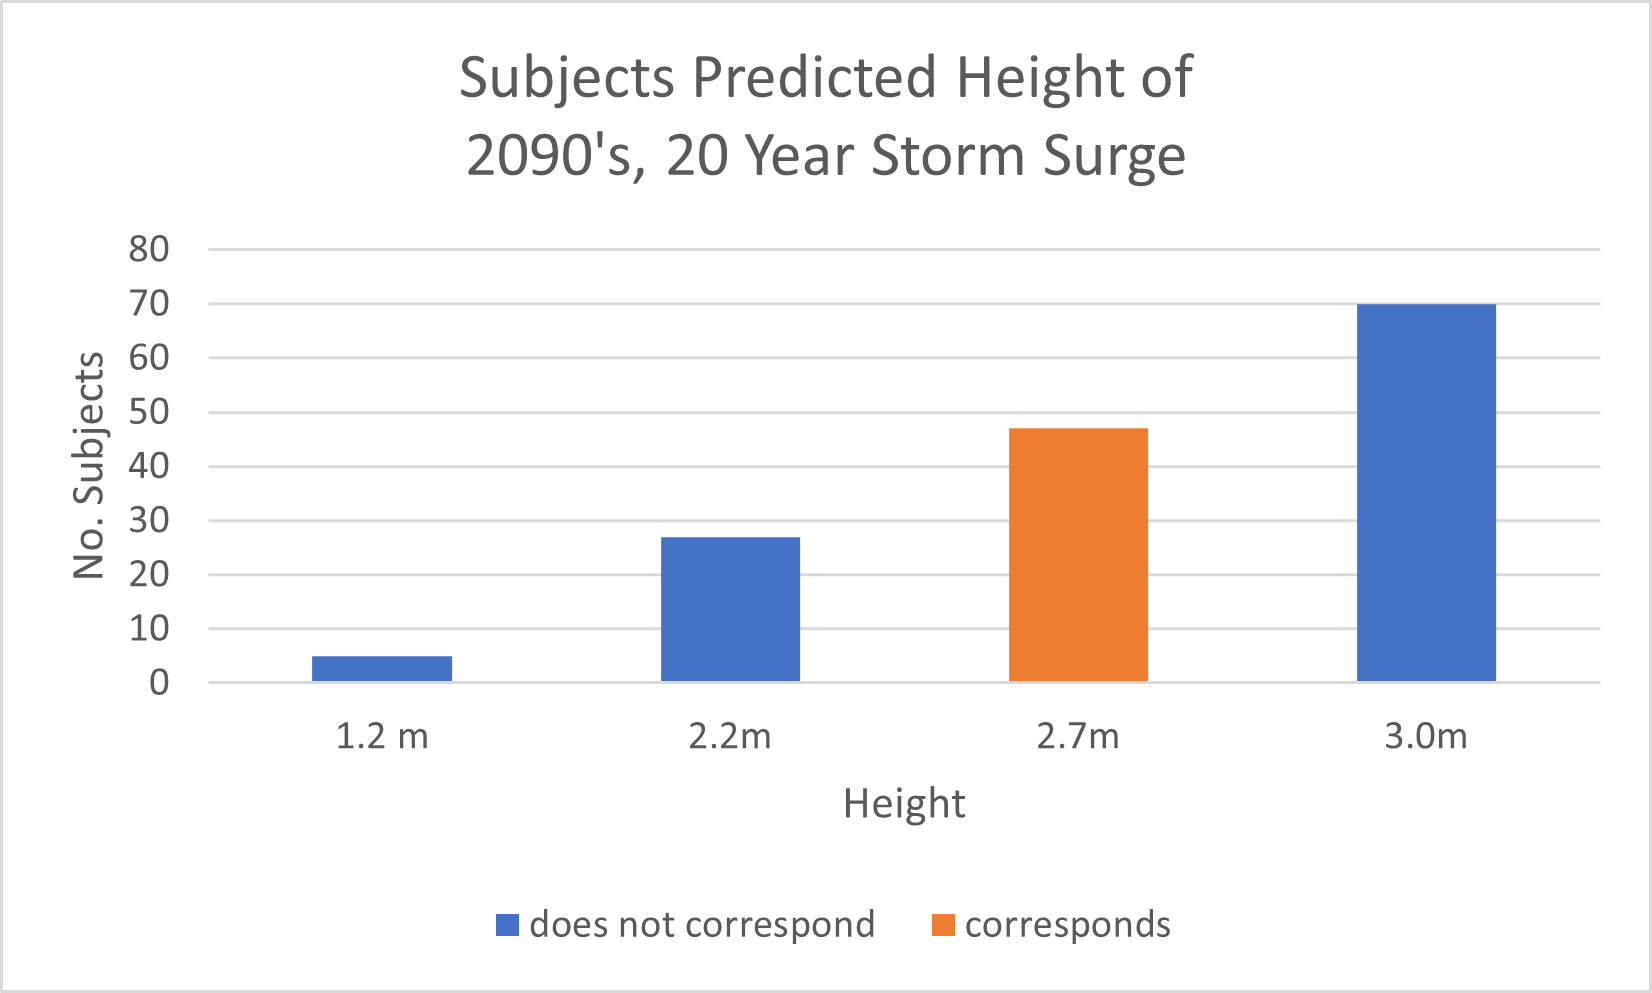
\includegraphics{fig_results/2090s 20yr ss answers.png}
    \caption{Subjects Predicted Height of 2090s' 20 year storm surge}{ The majority of subjects chose the highest value with 70 subjects choosing 3.0m as the predicted height of the storm surge. 47 subjects chose 2.7m which is the value which corresponds with models by (\cite{kartverket_se_2021}). 27 subjects chose 2.2m and only 5 subjects chose 1.2m}
    \label{fig:2090-stormsurge-answers}
\end{figure}
\paragraph{}
The most popular prediction was that the storm surge in 2090 will be 3.0m (46\%). Just over 30 \% chose 2.7m which is the value which corresponds with models from \cite{kartverket_se_2021}. This means that most people thought the sea level extreme associated with the 20 year storm surge in 2090 is higher than it is currently projected to be. The change of height for the 20 year storm surge predicted for 2090 is only 50cm higher than the current 20 year storm surge (\cite{kartverket_se_2021}). 
\paragraph{}

Figure \ref{fig:slr_future} shows the subjects predictions for how sea level will change in the next 30 years. 

\begin{figure}[H]
    \centering
    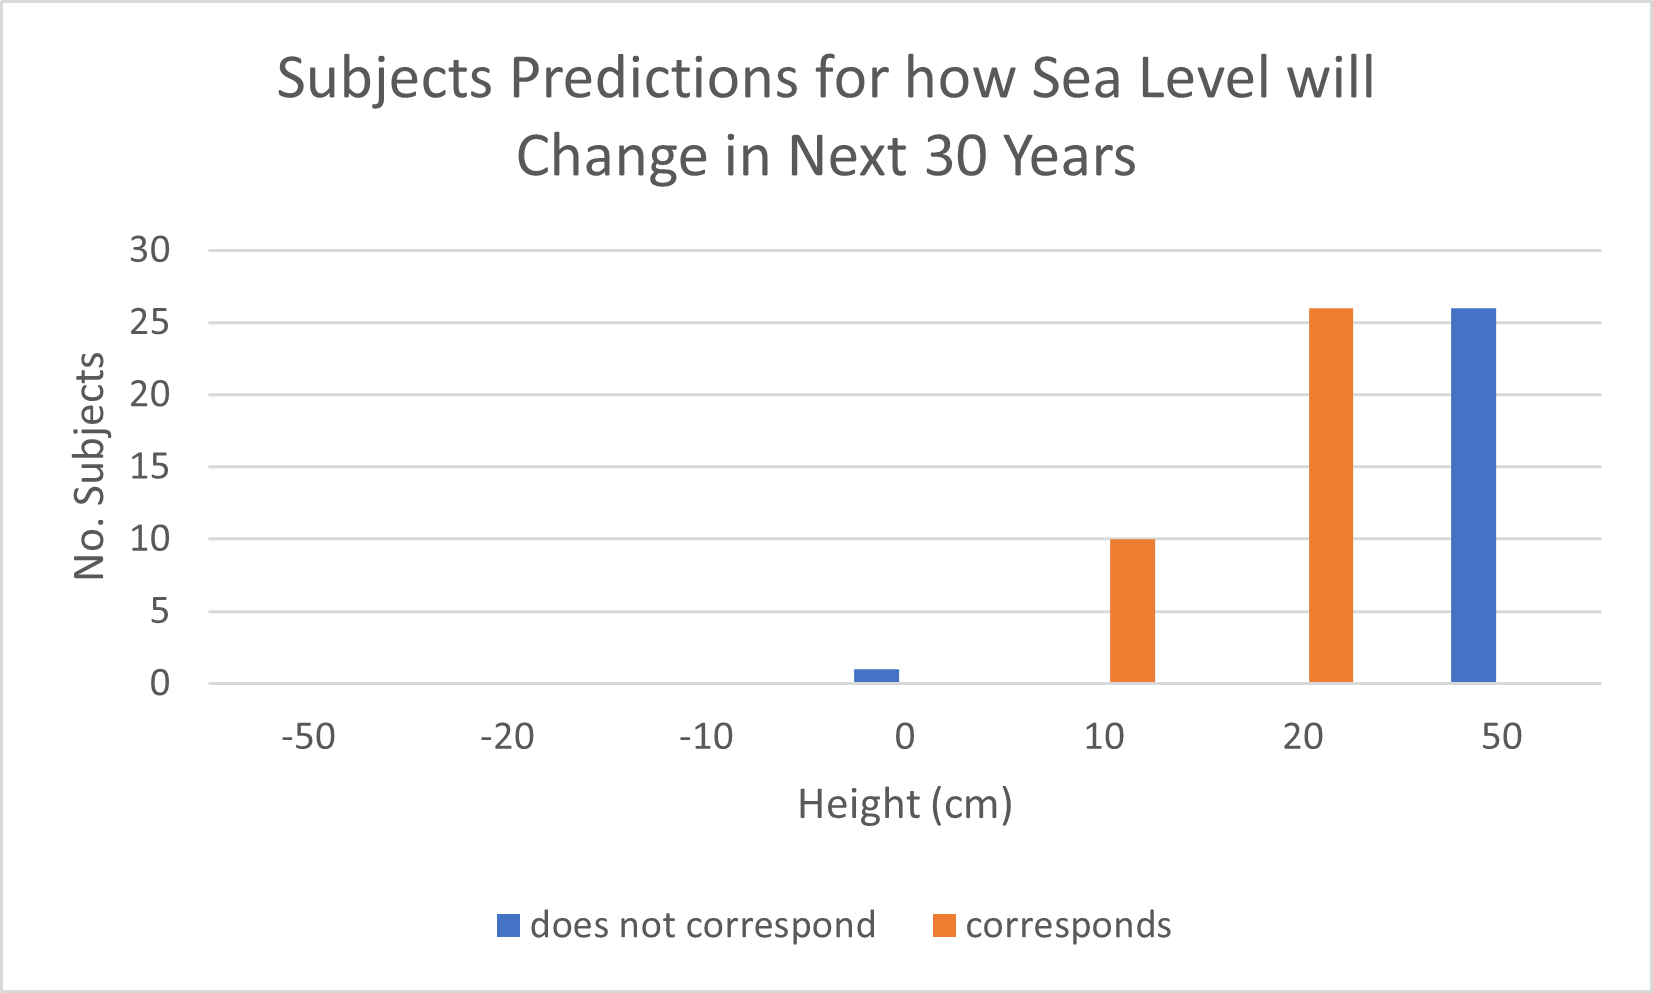
\includegraphics{fig_results/slr-future.png}
    \caption{Subjects Predictions of Sea Level Changes in Trondheim 2022-2052}{Only 147 subjects answered for this question, unlike every other question where all subjects answered (153). No subjects believed the sea level will decrease over the next 30 years. One subject answered that it will stay the same, with every other subject choosing that it will rise by some level }
    \label{fig:slr_future}
\end{figure}

There is strong uncertainty with this measurement in models, due to the difficulty of predicting emission patterns over the next 30 years and related glacio-isostatic uplift as they are dependent on global government policy (\cite{hanssen-bauer_climate_2017}; \cite{kartverket_se_2021}). Nevertheless, an estimation of 20cm or 10cm rise for Trondheim is in line with (\cite{kartverket_se_2021}) which uses the upper emissions pathways from the IPCC. Over half of the subjects chose a value which is in line with models from (\cite{kartverket_se_2021}). However, equal numbers of subjects, 26 , chose 50cm as chose 20cm,  which is not in line with these models. Almost all subjects answered that sea level will rise in the next 30 years, though six subjects chose not to answer this question.  

As shown in the survey in appendix C, figure \ref{fig:slr_future} and figure \ref{fig:slr_past} display results from questions which were purely numerical answers. There were no edited photographs to show the simulated SLEs.
\paragraph{}


\begin{figure}[H]
    \centering
    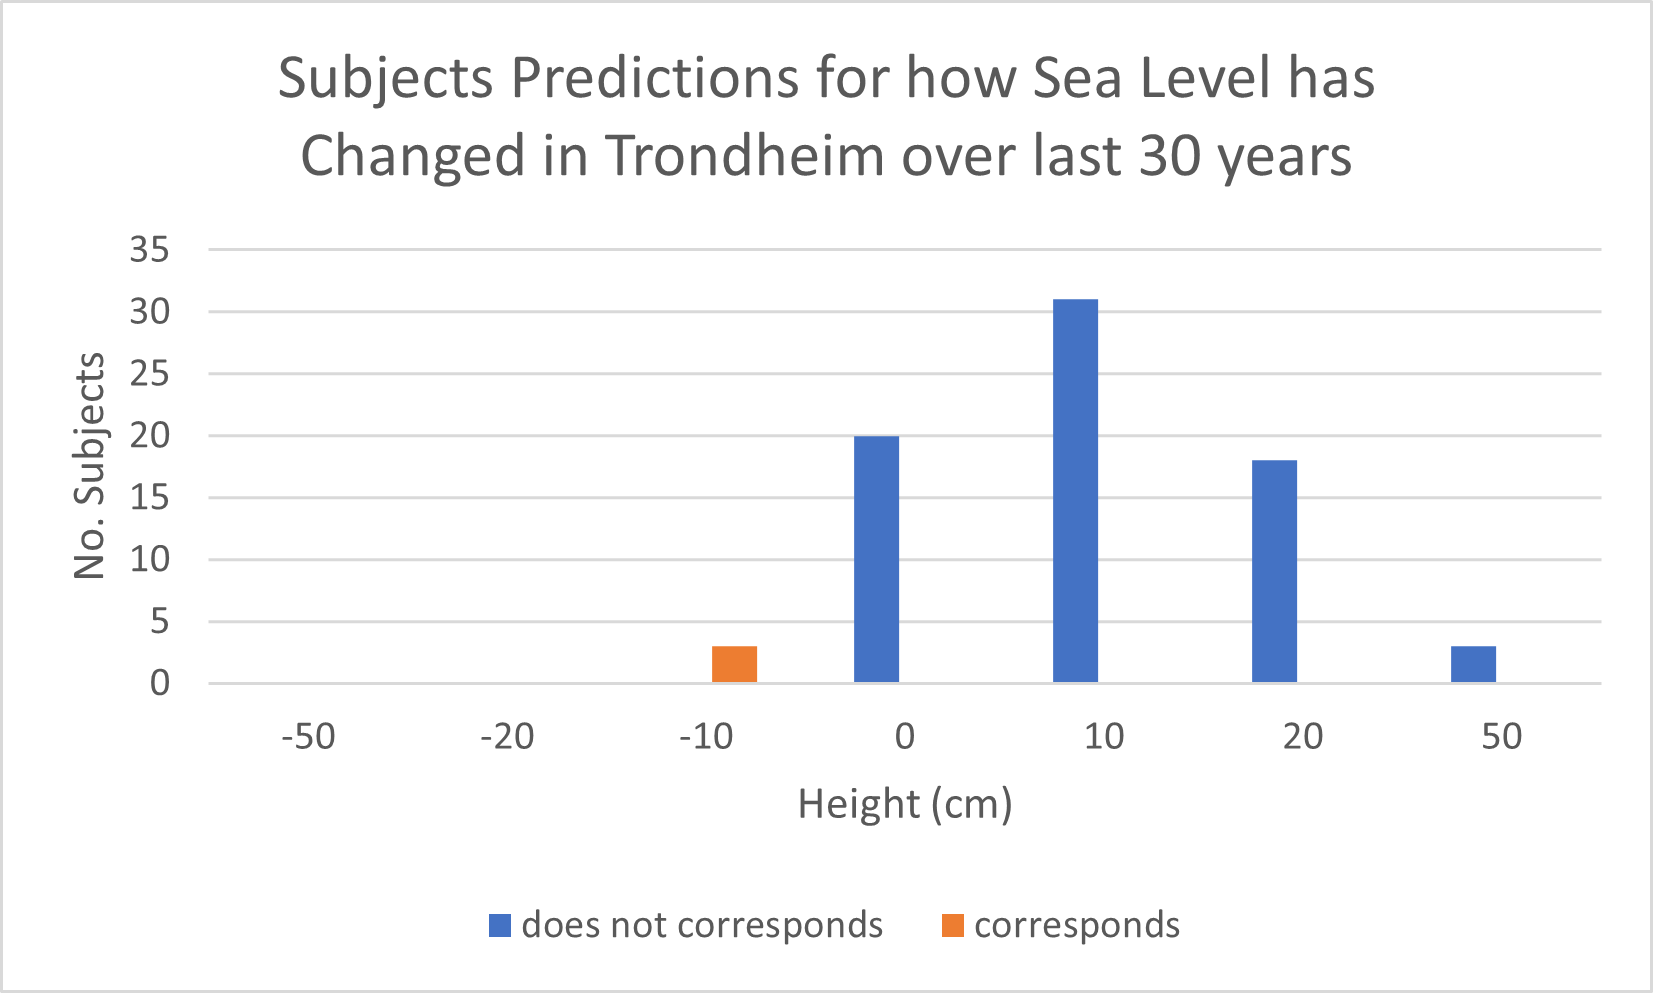
\includegraphics{fig_results/slr-past.png}
    \caption{Subjects Predictions for Sea Level Changes in Trondheim 1992-2022}{ Only 3 subjects selected that sea level has decreased in the last 30 years, the answer which corresponds with models from \cite{kartverket_se_2021}. 20 subjects answered that sea level had not changed over this time. While 31 subjects answered that it had risen by 10 cm. 18 subjects answered that it had risen by 20 cm and 3 answered that it had risen by 50 cm. 52 subjects answered that sea level had risen over the last 30 years. }
    \label{fig:slr_past}
\end{figure}

Figure \ref{fig:slr_past} shows the subjects predictions for how sea level has changed in Trondheim over the last 30 years. The certainty for the models presented here is high, as they are based off recordings not projections. Unlike subjects responses, sea level appears to have decreased in Trondheim over the last 30 years (\cite{tides_high_2022}).
\paragraph{}

Figure \ref{fig:aware_all_qs} is a combination of all results thus far in this section on awareness. This was the first attempt to determine awareness of subjects from the results of this survey

\begin{figure}[H]
    \centering
    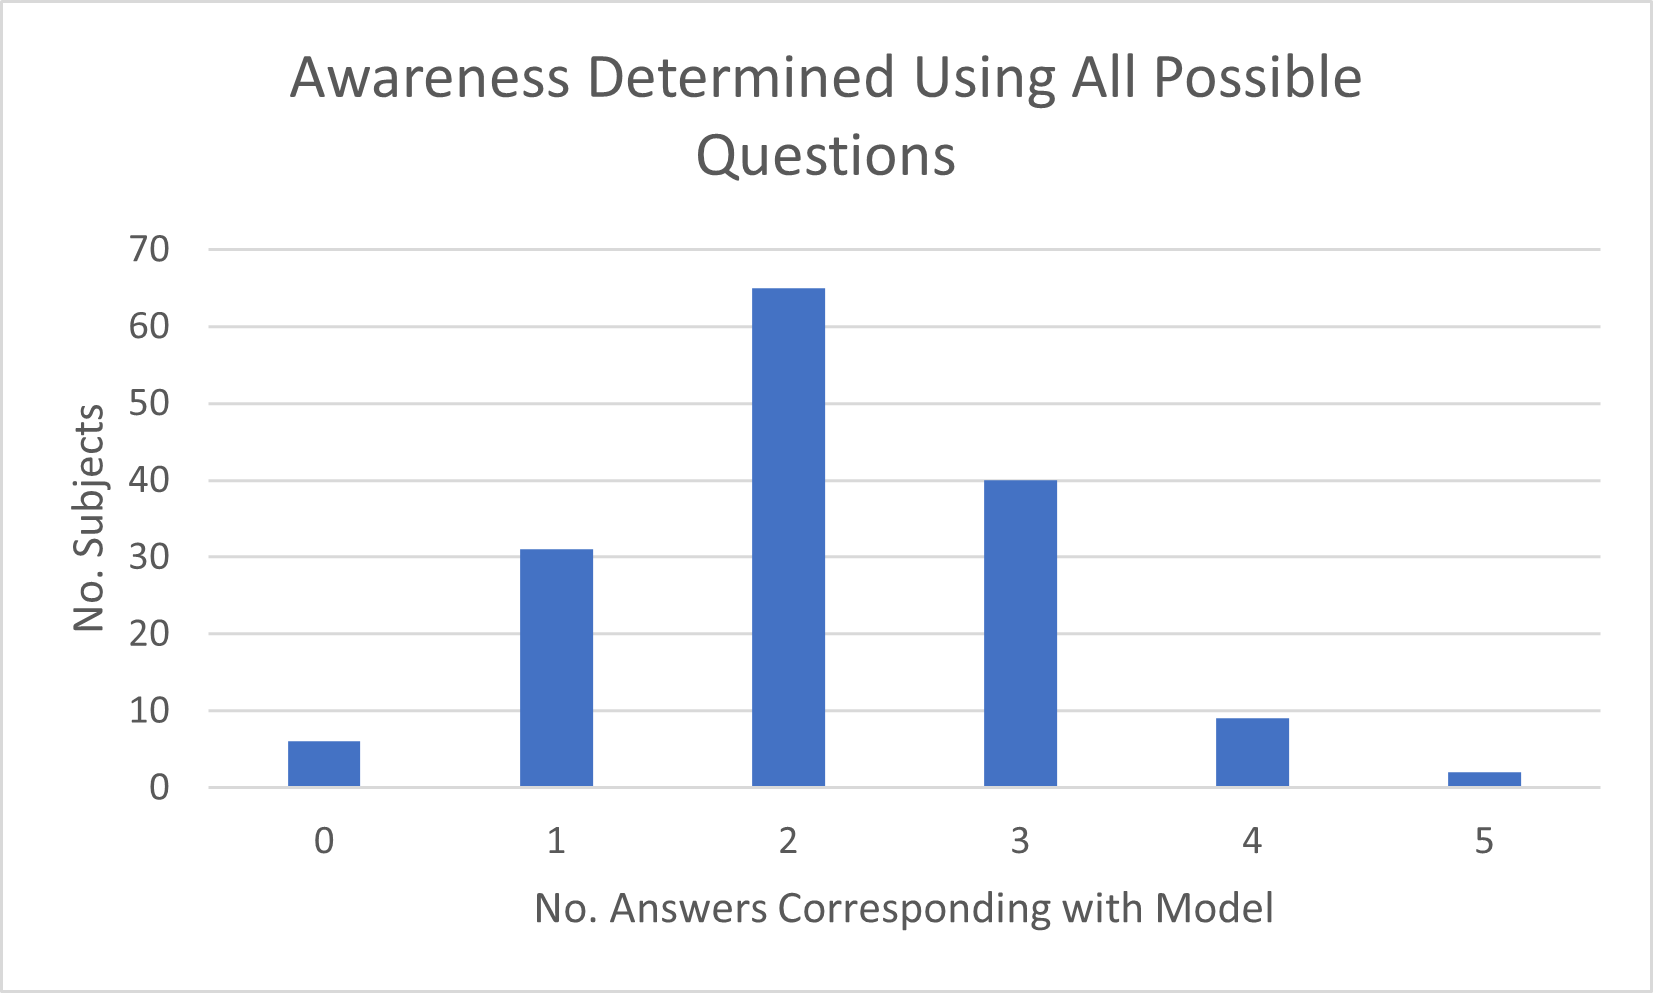
\includegraphics{fig_results/aware_all.png}
    \caption{Awareness Determined using all Possible Survey Questions}{All five questions from the survey on awareness to SLEs was used (three questions with a choice of simulated water level images and two with purely numerical options). Only 2 subjects had all answers corresponding with the models from (\cite{kartverket_se_2021}). 9 subjects had 4 answers corresponding, 40 subjects had 3 answers corresponding, 65 subjects had 2 answers corresponding, 31 subjects had 1 answer corresponding and 6 subjects had no answers corresponding. }
    \label{fig:aware_all_qs}
\end{figure}
\paragraph{}

Awareness determination considering all answers related to questions was deemed to be not the most suitable for analysing factors related to awareness (section \ref{discuss-aware}). For this reason, another determination of awareness was created utilising only the questions which had pictures of the simulated water levels, as discussed further in chapter 6 (section \ref{discuss-aware}). 
\paragraph{}

Figure \ref{fig:aware_all_edited_photo} shows determination of awareness considering the questions which utilised edited photographs, excluding the questions which were purely numeric. 

\begin{figure}[H]
    \centering
    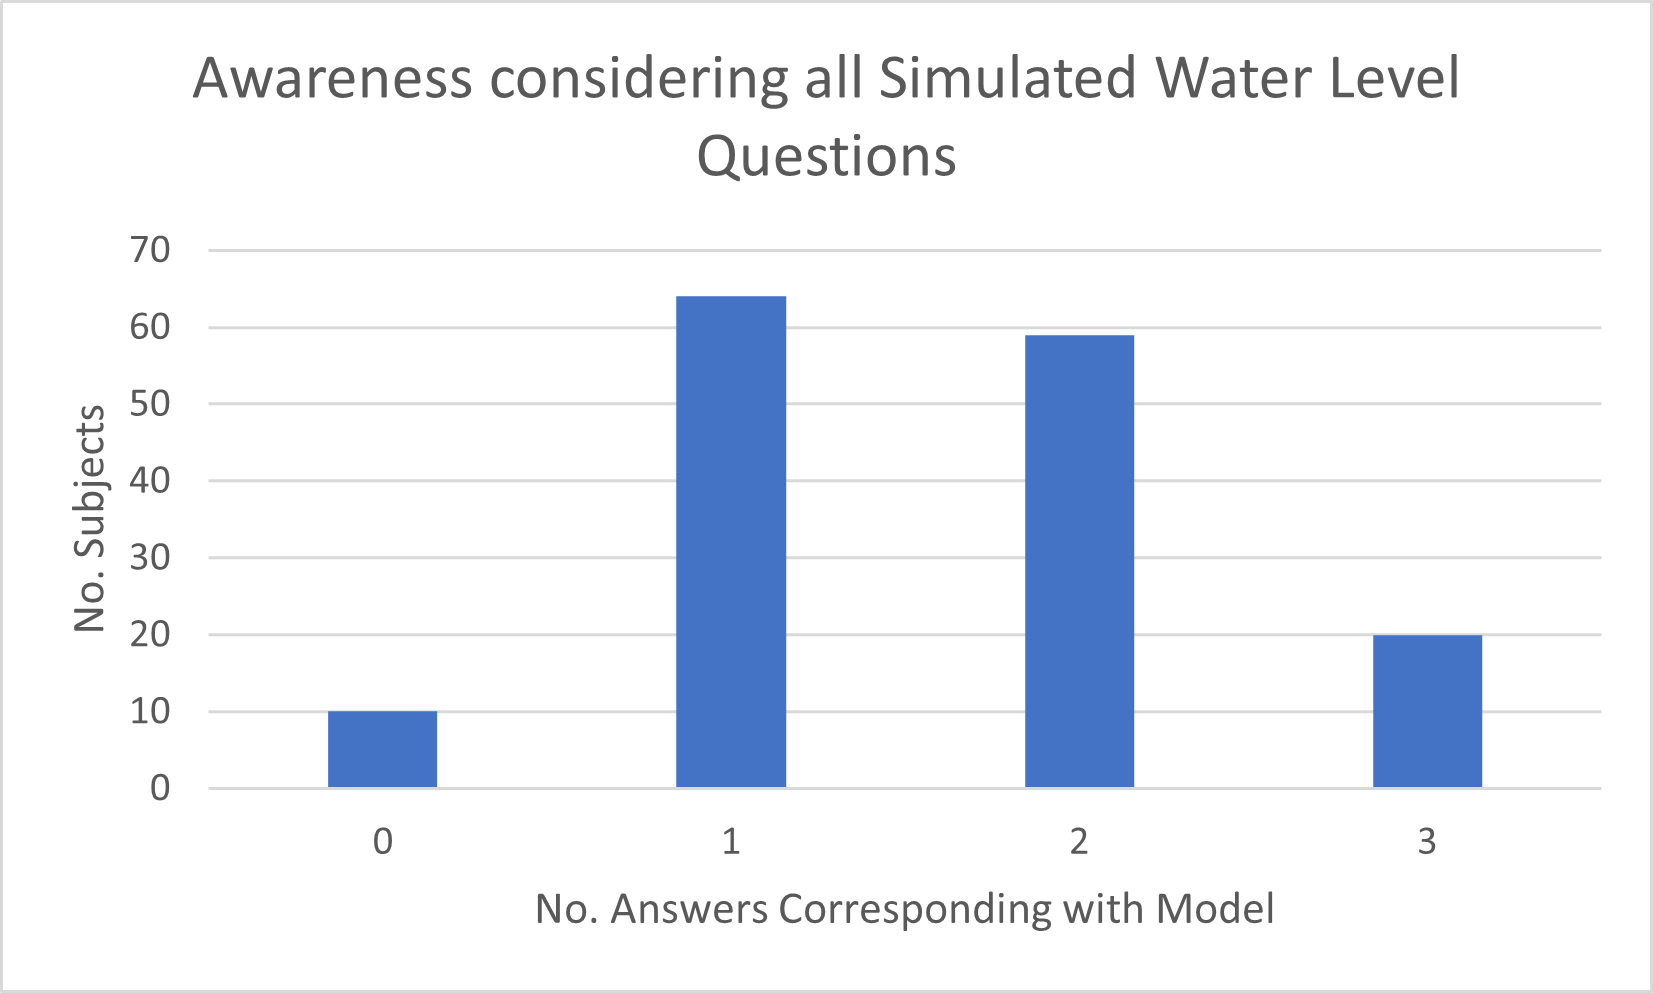
\includegraphics{fig_results/Awareness_ all_simulation_pictures_qs.png}
    \caption{Awareness Considering all Visually Simulated Water Level Questions}{ 10 subjects had no answers corresponding with the models from (\cite{kartverket_se_2021}), 20 subjects responded with every answer corresponding with the model for these questions. 64 subjects responded to one of the four questions with answers which corresponded with the models. 59 subjects responded with 2 answers which corresponded with the models. }
    \label{fig:aware_all_edited_photo}
\end{figure}


The results here are more evenly spread than in figure \ref{fig:aware_all_qs}, with the majority of subjects classing as somewhat aware. 
\paragraph{}
 


\paragraph{}
As shown by the focus group there is issues with just requesting a numeric value from subjects (section \ref{result-pilot-focus}). There appears to be a higher potential connection for many individuals, including emotional impact, when using pictures rather than numbers. 

\section{Factors Affecting Subjects' Awareness}
  

\subsection{Shapiro Test Results}

During exploratory analysis, only two factors appeared normally distributed. These factors came from the questions " What is your level of interest in sea level extremes?" (Interest Level) and "Where do you get information about climate change?", specifically how many sources the subjects selected (Info Climate Sum).   To investigate whether these factors were truly normally distributed, a Shapiro test was carried out following \cite{royston_extension_1982}. The results from the question on "How would flooding associated with sea level extremes in this area affect you?" was also investigated using this method.  An assumption of alpha value of 0.05 was determined meaningful (\cite{royston_extension_1982}). This means if the p-value created during this test is below 0.05 then the null hypothesis is rejected. This does leave a 5 \% chance of error. The results from the Shapiro test can be seen in table \ref{table:shapiro_test_results} and this determines that none of the variables were normally distributed. 

\begin{table}[H]
    \centering
    \begin{tabular}{|l|l|l|l|}
    \hline
         \textbf{ Variable } &  \textbf{W-value}& \textbf{ P-Value}& \textbf{Distribution}\\ \hline
       Interest Level & 0.89332 & 4.343e-09 & Skewed \\ \hline
         Info Climate Sum  & 0.95721 & 0.0001159 & Skewed \\ \hline
        Flood Impact & 0.87779 & 6.681e-10 & Skewed \\ \hline
     \end{tabular}
    \caption{Shapiro Test Results.} {The alpha value was assigned 0.05, meaning that if the p-value is below 0.05 then the null hypothesis that this factor is not normally distributed was rejected. This leaves a 5 \% chance of error. Each of these factors p-value is below 0.05 meaning that their distribution was deemed skewed. Interest Level is when subjects self-identified their interest level in SLEs, ranging from professional interest to no interest. Info Climate Sum is the total of how many different sources subjects used to gather information about the climate. Flood impact is what the subjects predicted a flood in the place would impact them ranging from no impact to significant impact. }
    \label{table:shapiro_test_results}
\end{table}
\paragraph{}


Table \ref{table:shapiro_test_results} shows that all variables and factors were skewed, including the important variable of awareness and interest level, influenced the choice of how to analyse dependency. As outlined in the method (section \ref{method-data-analysis}) Kruskal Wallis Rank Sum Tests were chosen due to the need to investigate multiple groups, upon one factor and having only measured each subject once. Figure \ref{fig:interest_level_SLE} displays the staked bar chart for the factor Interest Level. The factor of flood impact is displayed with the staked bar chart in Figure \ref{fig:flood_impact_pred}. Table \ref{table:sum_stats_info_climate_access} gives all the factors associated with the question "Where do you get information about climate change?".

\subsection{Kruskal Wallis Rank Sum Test Results}
The results from Kruskal Wallis Rank Sum Test conducted using the RStudio package based off \cite{hollander_nonparametric_2014} are outlined below.  An alpha value of 0.05 was chosen before these tests were carried out (\cite{hollander_nonparametric_2014}). This means there is a 5 \% chance of error when determining dependency of factors against the variable of awareness.
\paragraph{}
For clarity, the statistical labels for the Kruskal Wallis Rank Sum test are quickly outlined. For each of the results below, the p-value is the probability that measures the evidence against the null hypothesis.  If the p-value is lower than the selected alpha-value (0.05), then the null hypothesis can be rejected. The alternative way that the null hypothesis can be rejected utilises the H-value, which is the test statistic. If the \textit{df}, which stands for degrees of freedom, which is the number of groups within that factor, minus one, (\cite{minitab_interpret_2022}), is over four and the h-value is particularly high this can assist in the rejection of the hypothesis. Statistical interpretation used guidance from \cite{minitab_interpret_2022}. This section displays the results using tables, if a cell is highlighted blue it has a potentially significant result.Why the cell is highlighted blue is always outlined in the text. 
\paragraph{}

Table \ref{kw_test_general_factors}5.6 shows that, for the determination of awareness considering all questions on awareness, none of the factors were classed as dependent, when using the Kruskal Wallis rank sum test with an alpha value of 0.05. 

\begin{table}[H]
    \centering
    \begin{tabular}{|l|l|l|l|}
    \hline
         ~ & \textbf{awareness A} & ~ & ~ \\ \hline
        \textbf{Factor} &\textit{p} value &\textit{h} value & \textit{df} \\ \hline
           Length of Knowledge & 0.73760 & 3.54770 & 6 \\ \hline
       Interest Level in SLE & 0.16920 & 6.43150 & 4 \\ \hline
        Concern about Climate & \cellcolor[HTML]{7df9ff} 0.05630 & \cellcolor[HTML]{7df9ff} 9.19960 & \cellcolor[HTML]{7df9ff} 4 \\ \hline
        Language of Survey & 0.2041 & 1.6129 & 1 \\ \hline
        Predicted Personal Impact of Flood & 0.7156 & 1.357 & 3 \\ \hline
    \end{tabular}
    \caption{Kruskal Wallis Test Results - General Factors.}{ "awareness A" means that for this determination of awareness, all five questions on awareness in the survey were included. Length of knowledge is how many years the subjects state they have knowledge of the places. Interest level in SLE represents the self-ranking of subjects from professional interest to no interest. Concern about Climate is self ranking of how concerned subjects are about climate change, from one to five. Language of survey, is whether the subjects chose to respond in Norwegian or English. Predicted Personal Impact of Flood is specifically for flooding in the research place and ranges from no impact to significant impact. }
    \label{kw_test_general_factors}
\end{table}

All the p-values were larger than the alpha value of 0.05. However, the p-value of Concern about Climate is 0.05630, highlighted in blue, is only just over.  If the alpha value was chosen to be 0.1, as is used in some studies (\cite{hollander_nonparametric_2014}), then this would be enough to reject the null hypothesis that concern about awareness is not dependent upon concern about climate. However, the h-value is exceptionally high and the \textit{df} is 4, meaning that, while not as confident as with a p-value rejection, the null hypothesis is still rejected (\cite{minitab_interpret_2022}). The result is that awareness appears dependent upon Concern about Climate. 
\paragraph{}


Table \ref{kw_test_com_membership} shows the Kruskal Wallis Test Results for the factors about the subjects community memberships. 


\begin{table}[H]
    \centering
    \begin{tabular}{|l|l|l|l|}
    \hline
         ~ & \textbf{awareness A} & ~ & ~ \\ \hline
        \textbf{Factor} &\textit{p} value &\textit{h} value & \textit{df} \\ \hline
        Sum of Community Memberships & 0.52060 & 4.20260 & 7 \\ \hline
        Marine worker & na & na & na \\ \hline
        Worker & 0.12310 & 2.37220 & 1 \\ \hline
        Resident & \cellcolor[HTML]{7df9ff} 0.01524 & 5.88900 & 1 \\ \hline
        Student & 0.55590 & 0.34691 & 1 \\ \hline
        Commuter & 0.44610 & 0.58063 & 1 \\ \hline
        Leisure User Land & 0.68790 & 0.16141 & 1 \\ \hline
        Leisure User water & 0.42120 & 0.64690 & 1 \\ \hline
        Other & 0.58620 & 0.29627 & 1 \\ \hline
    \end{tabular}
    \caption{Kruskal Wallis Test Results - Community Membership as Factor}{ "awareness A" means that for this determination of awareness, all five questions on awareness in the survey were included. Sum of Community Memberships is how many communities did the subjects select in the survey. Marine worker is whether the subject considered themselves a marine worker. This had no responses. Community memberships also included worker, resident, student, commuter, leisure user land, leisure user water and other. The Other community membership was where the subjects self-identified their community: the most common response was tourist, with sailor coming next. The values highlighted in blue are statistically significant.}
    \label{kw_test_com_membership}
\end{table}
Resident is the only value which is highlighted in table \ref{kw_test_com_membership} as it is the only significant result when utilising an alpha value of 0.05. The factor of resident has a P-value of 0.01524, meaning the differences between the medians are statistically significant. This allows the rejection of the null hypothesis and the acceptance of the positive hypothesis that awareness is dependent on residency. 
\paragraph{}

Table \ref{kw_test_info_place} shows the Kruskal Wallis Test Results on the factors covering Information Sources for Place. Two forms of determining awareness are used as predictors. "awareness A", where all five questions on awareness in the survey were included and "awareness B", where only the questions which utilised edited photographs are used to determine awareness.

\begin{table}[H]
    \centering
    \begin{tabular}{|l|l|l|l|l|l|l|}
    \hline
       & \textbf{awareness A} & ~ & ~ & \textbf{awareness B} & ~ & ~ \\ \hline
       Factor &\textit{p}value &\textit{h}value & \textit{df} &\textit{p}value &\textit{h}value & \textit{df} \\ \hline
        Sum of Sources  & 0.44600 & 6.85110 & 7 & 0.45040 & 6.79650 & 7 \\ \hline
        Personal Observation & 0.22730 & 1.45790 & 1 & 0.36470 & 0.82162 & 1 \\ \hline
        Family & 0.78550 & 0.07406 & 1 & 0.81340 & 0.05572 & 1 \\ \hline
        Friend & 0.27580 & 1.18780 & 1 & 0.30200 & 1.06520 & 1 \\ \hline
        Newspaper & 0.74490 & 0.10583 & 1 & 0.48500 & 0.48765 & 1 \\ \hline
        TV & 0.87330 & 0.02542 & 1 & 0.33420 & 0.93237 & 1 \\ \hline
        Social Media & 0.48540 & 0.48671 & 1 & 0.95090 & 0.00379 & 1 \\ \hline
        Membership of Organisation  & 0.67530 & 0.17550 & 1 & 0.70980 & 0.13848 & 1 \\ \hline
        Municipality & 0.82590 & 0.04839 & 1 & 0.12790 & 0.57600 & 1 \\ \hline
        \hline
    \end{tabular}
    \caption{Kruskal Wallis Test Results - Information Sources for Place as Factor}{  "Awareness A" means that for this determination of awareness the three questions on awareness utilising edited photographs were included, which display awareness of the tide and present and future storm surges.  "Awareness B" excludes the future storm surge response and only considers the present storm surge and tide.  The sum of sources is the total number of sources each subject selected as where they gather information about place from. These sources are personal observation, family, friend, newspapers, TV, social media, via membership of organisations and the Municipality. The values highlighted in blue are statistically significant. }
    \label{kw_test_info_place}
\end{table}

There were no significant values, meaning that for each of these hypotheses the null hypotheses was accepted.
\paragraph{}
Table \ref{kwtest_info_climate} shows the Kruskal Wallis Test Results on the factors Information Sources for Climate. As with Table \ref{kw_test_info_place}, two determinations of awareness are used as predictors.



\begin{table}[H]
    \centering
    \begin{tabular}{|l|l|l|l|l|l|l|}
    \hline
        & \textbf{awareness A} & ~ & ~ & \textbf{awareness B} & ~ & ~ \\ \hline
        Factor &\textit{p}value &\textit{h}value & \textit{df} & \textit{p}value &\textit{h}value & \textit{df} \\ \hline
        Sum of Sources & 0.91220 & 3.32660 & 8 & 0.45218 & 8.12040 & 8 \\ \hline
        Personal Observation & 0.11750 & 2.45020 & 1 & 0.24550 & 1.34870 & 1 \\ \hline
        Family & \cellcolor[HTML]{7df9ff} 0.00481 & 0.94470 & 1 & 0.56970 & 0.32313 & 1 \\ \hline
        Friend & 0.82460 & 0.04910 & 1 & 0.63010 & 0.23186 & 1 \\ \hline
        Newspaper & 0.09036 & 2.86790 & 1 & \cellcolor[HTML]{7df9ff} 0.01218 & 6.24830 & 1 \\ \hline
        TV & 0.61230 & 0.25689 & 1 & 0.75000 & 0.10154 & 1 \\ \hline
        Social Media & 0.74950 & 0.10960 & 1 & 0.92830 & 0.00809 & 1 \\ \hline
        Membership of Organisation & 0.30270 & 1.06220 & 1 & 0.27500 & 1.91500 & 1 \\ \hline
        Peer Reviewed Publications  & 0.88040 & 0.02650 & 1 & 0.12390 & 2.36760 & 1 \\ \hline
        Formal Education & 0.64850 & 0.20779 & 1 & \cellcolor[HTML]{7df9ff} 0.02438 & 5.06770 & 1 \\ \hline
    \end{tabular}
    \caption{Kruskal Wallis Test Results - Information Sources for Climate as Factor}{ "Awareness A" means that for this determination of awareness the three questions on awareness utilising edited photographs were included, which display awareness of the tide and present and future storm surges.  "Awareness B" excludes the future storm surge response and only considers the present storm surge and tide.  The sum of sources is the total number of sources each subject selected as from where they gather information about changes to the climate. These sources are personal observation, family, friend, newspapers, TV, social media, via membership of organisations, peer reviewed publications and formal education. The values highlighted in blue are statistically significant. }
    \label{kwtest_info_climate}
\end{table}

For the determination of awareness which considered all five possible questions, Family is a significant factor. This means that this determination of awareness appears dependent on family as a sources of observation. This result is discussed later in the context that 25 subjects have a personal connection to the researcher.
\paragraph{}
For the determination of awareness which only utilised the edited photograph questions, both the information source of newspaper and formal education were significant.
\paragraph{}
Table \ref{kwtest_place} shows the Kruskal Wallis Test Results on the factors of Place subjects responded on. These places had varied physical vulnerability as outlined in table \ref{table:research_site} in the background.

\begin{table}[H]
    \centering
    \begin{tabular}{|l|l|l|l|l|l|l|}
    \hline

   
 ~ & \textbf{awareness A} & ~ & \textbf{awareness B} & ~ & ~ &\\\hline
        \textbf{Factor} &\textit{p} value &\textit{h} value & \textit{df} &\textit{p}value &\textit{h}value & \textit{df}\\ \hline
         Brattøra & 0.1044  & 2.6364 & 1 & 0.771 & 0.084739 &1\\ \hline
        Grillstad & 0.1815 & 1.7855 & 1 & 0.1565 & 2.008 & 1 \\ \hline
       Skansen & 0.09349 & 2.8133 & 1 & 0.05527 & 3.6738 & 1\\ \hline
         Nidelva & 0.2472 & 1.3388 & 1 & 0.9523 &  0.0035714 & 1\\ \hline
    \end{tabular}
    \caption{Kruskal Wallis Test Results - Place as Factor}{ "Awareness A" means that for this determination of awareness the three questions on awareness utilising edited photographs were included, which display awareness of the tide and present and future storm surges.  "Awareness B" excludes the future storm surge response and only considers the present storm surge and tide.  Brattøra, Grillstad, Skansen and Nidelva are the places considered.}
    \label{kwtest_place}
\end{table}
None of the factors of each of the places have a statistically distinct median. This means the null hypothesis is accepted and awareness is not considered dependent on the variable of place. 
  How the non-parametric hypothesis testing of Kruskal Wallis Rank Sum tests relate to the original hypotheses it outlined at the end of the discussion section (section \ref{RQ3 - finding}).   
\paragraph{}

  









